
%% Support sites:
%% http://www.michaelshell.org/tex/ieeetran/
%% http://www.ctan.org/pkg/ieeetran
%% and
%% http://www.ieee.org/


\documentclass[conference]{IEEEtran}
\usepackage{xltxtra}
\usepackage{xunicode}
\usepackage{fontspec}

\usepackage{polyglossia}
\setmainlanguage{english}
\setotherlanguage{thai}
\setmainfont{Times New Roman}
\setsansfont{Arial}
\newfontfamily\thaifont[Scale=1.2]{THSarabunNew}
\newfontfamily\thaifontsf[Scale=1.2]{THSarabunNew}


%\defaultfontfeatures{Scale=MatchLowercase}
%\setmainfont[Scale=1.0]{Kinnari}
\XeTeXlinebreaklocale “th_TH”



%\setmainfont[Script=Thai]{Loma}
\setmonofont[Script=Thai]{TlwgTypewriter}
% Some very useful LaTeX packages include:
% (uncomment the ones you want to load)

%\usepackage{fonts-tlwg}

% *** MISC UTILITY PACKAGES ***
%
%\usepackage{ifpdf}
% Heiko Oberdiek's ifpdf.sty is very useful if you need conditional
% compilation based on whether the output is pdf or dvi.
% usage:
% \ifpdf
%   % pdf code
% \else
%   % dvi code
% \fi
% The latest version of ifpdf.sty can be obtained from:
% http://www.ctan.org/pkg/ifpdf
% Also, note that IEEEtran.cls V1.7 and later provides a builtin
% \ifCLASSINFOpdf conditional that works the same way.
% When switching from latex to pdflatex and vice-versa, the compiler may
% have to be run twice to clear warning/error messages.


\usepackage{url}
\usepackage{multirow}



% *** CITATION PACKAGES ***
%
\usepackage{cite}
% cite.sty was written by Donald Arseneau
% V1.6 and later of IEEEtran pre-defines the format of the cite.sty package
% \cite{} output to follow that of the IEEE. Loading the cite package will
% result in citation numbers being automatically sorted and properly
% "compressed/ranged". e.g., [1], [9], [2], [7], [5], [6] without using
% cite.sty will become [1], [2], [5]--[7], [9] using cite.sty. cite.sty's
% \cite will automatically add leading space, if needed. Use cite.sty's
% noadjust option (cite.sty V3.8 and later) if you want to turn this off
% such as if a citation ever needs to be enclosed in parenthesis.
% cite.sty is already installed on most LaTeX systems. Be sure and use
% version 5.0 (2009-03-20) and later if using hyperref.sty.
% The latest version can be obtained at:
% http://www.ctan.org/pkg/cite
% The documentation is contained in the cite.sty file itself.






% *** GRAPHICS RELATED PACKAGES ***
%
%\ifCLASSINFOpdf
%   \usepackage[pdftex]{graphicx}
\usepackage{graphicx}
%  % declare the path(s) where your graphic files are
%  % \graphicspath{{../pdf/}{../jpeg/}}
%  % and their extensions so you won't have to specify these with
%  % every instance of \includegraphics
%   \DeclareGraphicsExtensions{.pdf,.jpeg,.png}
%\else
%  % or other class option (dvipsone, dvipdf, if not using dvips). graphicx
%  % will default to the driver specified in the system graphics.cfg if no
%  % driver is specified.
%   \usepackage[dvips]{graphicx}
%  % declare the path(s) where your graphic files are
%  % \graphicspath{{../eps/}}
%  % and their extensions so you won't have to specify these with
%  % every instance of \includegraphics
%   \DeclareGraphicsExtensions{.eps,.jpeg,.png}
%\fi
% graphicx was written by David Carlisle and Sebastian Rahtz. It is
% required if you want graphics, photos, etc. graphicx.sty is already
% installed on most LaTeX systems. The latest version and documentation
% can be obtained at: 
% http://www.ctan.org/pkg/graphicx
% Another good source of documentation is "Using Imported Graphics in
% LaTeX2e" by Keith Reckdahl which can be found at:
% http://www.ctan.org/pkg/epslatex
%
% latex, and pdflatex in dvi mode, support graphics in encapsulated
% postscript (.eps) format. pdflatex in pdf mode supports graphics
% in .pdf, .jpeg, .png and .mps (metapost) formats. Users should ensure
% that all non-photo figures use a vector format (.eps, .pdf, .mps) and
% not a bitmapped formats (.jpeg, .png). The IEEE frowns on bitmapped formats
% which can result in "jaggedy"/blurry rendering of lines and letters as
% well as large increases in file sizes.
%
% You can find documentation about the pdfTeX application at:
% http://www.tug.org/applications/pdftex





% *** MATH PACKAGES ***
%
%\usepackage{amsmath}
% A popular package from the American Mathematical Society that provides
% many useful and powerful commands for dealing with mathematics.
%
% Note that the amsmath package sets \interdisplaylinepenalty to 10000
% thus preventing page breaks from occurring within multiline equations. Use:
%\interdisplaylinepenalty=2500
% after loading amsmath to restore such page breaks as IEEEtran.cls normally
% does. amsmath.sty is already installed on most LaTeX systems. The latest
% version and documentation can be obtained at:
% http://www.ctan.org/pkg/amsmath





% *** SPECIALIZED LIST PACKAGES ***
%
%\usepackage{algorithmic}
% algorithmic.sty was written by Peter Williams and Rogerio Brito.
% This package provides an algorithmic environment fo describing algorithms.
% You can use the algorithmic environment in-text or within a figure
% environment to provide for a floating algorithm. Do NOT use the algorithm
% floating environment provided by algorithm.sty (by the same authors) or
% algorithm2e.sty (by Christophe Fiorio) as the IEEE does not use dedicated
% algorithm float types and packages that provide these will not provide
% correct IEEE style captions. The latest version and documentation of
% algorithmic.sty can be obtained at:
% http://www.ctan.org/pkg/algorithms
% Also of interest may be the (relatively newer and more customizable)
% algorithmicx.sty package by Szasz Janos:
% http://www.ctan.org/pkg/algorithmicx




% *** ALIGNMENT PACKAGES ***
%
%\usepackage{array}
% Frank Mittelbach's and David Carlisle's array.sty patches and improves
% the standard LaTeX2e array and tabular environments to provide better
% appearance and additional user controls. As the default LaTeX2e table
% generation code is lacking to the point of almost being broken with
% respect to the quality of the end results, all users are strongly
% advised to use an enhanced (at the very least that provided by array.sty)
% set of table tools. array.sty is already installed on most systems. The
% latest version and documentation can be obtained at:
% http://www.ctan.org/pkg/array


% IEEEtran contains the IEEEeqnarray family of commands that can be used to
% generate multiline equations as well as matrices, tables, etc., of high
% quality.




% *** SUBFIGURE PACKAGES ***
%\ifCLASSOPTIONcompsoc
%  \usepackage[caption=false,font=normalsize,labelfont=sf,textfont=sf]{subfig}
%\else
%  \usepackage[caption=false,font=footnotesize]{subfig}
%\fi
% subfig.sty, written by Steven Douglas Cochran, is the modern replacement
% for subfigure.sty, the latter of which is no longer maintained and is
% incompatible with some LaTeX packages including fixltx2e. However,
% subfig.sty requires and automatically loads Axel Sommerfeldt's caption.sty
% which will override IEEEtran.cls' handling of captions and this will result
% in non-IEEE style figure/table captions. To prevent this problem, be sure
% and invoke subfig.sty's "caption=false" package option (available since
% subfig.sty version 1.3, 2005/06/28) as this is will preserve IEEEtran.cls
% handling of captions.
% Note that the Computer Society format requires a larger sans serif font
% than the serif footnote size font used in traditional IEEE formatting
% and thus the need to invoke different subfig.sty package options depending
% on whether compsoc mode has been enabled.
%
% The latest version and documentation of subfig.sty can be obtained at:
% http://www.ctan.org/pkg/subfig




% *** FLOAT PACKAGES ***
%
%\usepackage{fixltx2e}
% fixltx2e, the successor to the earlier fix2col.sty, was written by
% Frank Mittelbach and David Carlisle. This package corrects a few problems
% in the LaTeX2e kernel, the most notable of which is that in current
% LaTeX2e releases, the ordering of single and double column floats is not
% guaranteed to be preserved. Thus, an unpatched LaTeX2e can allow a
% single column figure to be placed prior to an earlier double column
% figure.
% Be aware that LaTeX2e kernels dated 2015 and later have fixltx2e.sty's
% corrections already built into the system in which case a warning will
% be issued if an attempt is made to load fixltx2e.sty as it is no longer
% needed.
% The latest version and documentation can be found at:
% http://www.ctan.org/pkg/fixltx2e


%\usepackage{stfloats}
% stfloats.sty was written by Sigitas Tolusis. This package gives LaTeX2e
% the ability to do double column floats at the bottom of the page as well
% as the top. (e.g., "\begin{figure*}[!b]" is not normally possible in
% LaTeX2e). It also provides a command:
%\fnbelowfloat
% to enable the placement of footnotes below bottom floats (the standard
% LaTeX2e kernel puts them above bottom floats). This is an invasive package
% which rewrites many portions of the LaTeX2e float routines. It may not work
% with other packages that modify the LaTeX2e float routines. The latest
% version and documentation can be obtained at:
% http://www.ctan.org/pkg/stfloats
% Do not use the stfloats baselinefloat ability as the IEEE does not allow
% \baselineskip to stretch. Authors submitting work to the IEEE should note
% that the IEEE rarely uses double column equations and that authors should try
% to avoid such use. Do not be tempted to use the cuted.sty or midfloat.sty
% packages (also by Sigitas Tolusis) as the IEEE does not format its papers in
% such ways.
% Do not attempt to use stfloats with fixltx2e as they are incompatible.
% Instead, use Morten Hogholm'a dblfloatfix which combines the features
% of both fixltx2e and stfloats:
%
% \usepackage{dblfloatfix}
% The latest version can be found at:
% http://www.ctan.org/pkg/dblfloatfix




% *** PDF, URL AND HYPERLINK PACKAGES ***
%
%\usepackage{url}
% url.sty was written by Donald Arseneau. It provides better support for
% handling and breaking URLs. url.sty is already installed on most LaTeX
% systems. The latest version and documentation can be obtained at:
% http://www.ctan.org/pkg/url
% Basically, \url{my_url_here}.




% *** Do not adjust lengths that control margins, column widths, etc. ***
% *** Do not use packages that alter fonts (such as pslatex).         ***
% There should be no need to do such things with IEEEtran.cls V1.6 and later.
% (Unless specifically asked to do so by the journal or conference you plan
% to submit to, of course. )


% correct bad hyphenation here
\hyphenation{op-tical net-works semi-conduc-tor}


\begin{document}
%
% paper title
% Titles are generally capitalized except for words such as a, an, and, as,
% at, but, by, for, in, nor, of, on, or, the, to and up, which are usually
% not capitalized unless they are the first or last word of the title.
% Linebreaks \\ can be used within to get better formatting as desired.
% Do not put math or special symbols in the title.
\title{Analyzing User Reviews in Thai Language\\ toward Features in Application}


% author names and affiliations
% use a multiple column layout for up to three different
% affiliations
\author{\IEEEauthorblockN{Boonyarit Deewattananon, Usa Sammapun}
\IEEEauthorblockA{Department of Computer Science, Faculty of Science\\
Kasetsart University, Bangkok, Thailand\\
Email: \{g5614401148,fsciusa\}@ku.ac.th}
}
%\and
%\IEEEauthorblockN{Usa Sammapun}
%\IEEEauthorblockA{Twentieth Century Fox\\
%Springfield, USA\\
%Email: fsciusa@ku.ac.th}
%}

% conference papers do not typically use \thanks and this command
% is locked out in conference mode. If really needed, such as for
% the acknowledgment of grants, issue a \IEEEoverridecommandlockouts
% after \documentclass

% for over three affiliations, or if they all won't fit within the width
% of the page, use this alternative format:
% 
%\author{\IEEEauthorblockN{Usa Sammapun\IEEEauthorrefmark{1},
%Boonyarit Deewattananon\IEEEauthorrefmark{2}}
%\IEEEauthorblockA{Department of Computer Science, Faculty of Science\\
%Kasetsart University, Bangkok, Thailand\\
%\IEEEauthorrefmark{1}fsciusa@ku.ac.th, \IEEEauthorrefmark{2}g5614401148@ku.ac.th}
%\IEEEauthorblockA{\IEEEauthorrefmark{3}Starfleet Academy, San Francisco, California 96678-2391\\
%Telephone: (800) 555--1212, Fax: (888) 555--1212}
%\IEEEauthorblockA{\IEEEauthorrefmark{4}Tyrell Inc., 123 Replicant Street, Los Angeles, California 90210--4321}
%}




% use for special paper notices
%\IEEEspecialpapernotice{(Invited Paper)}




% make the title area
\maketitle

% As a general rule, do not put math, special symbols or citations
% in the abstract
\begin{abstract}
The abstract goes here. limited to the maximum of 6 pages of A4 form in PDF format. an abstract of about 100 words. The authors’ names and affiliations, postal addresses, telephones, fax numbers and e-mail addresses must be omitted.
\end{abstract}

% no keywords




% For peer review papers, you can put extra information on the cover
% page as needed:
% \ifCLASSOPTIONpeerreview
% \begin{center} \bfseries EDICS Category: 3-BBND \end{center}
% \fi
%
% For peerreview papers, this IEEEtran command inserts a page break and
% creates the second title. It will be ignored for other modes.
\IEEEpeerreviewmaketitle

%\section{Introduction}
% no \IEEEPARstart
% You must have at least 2 lines in the paragraph with the drop letter
% (should never be an issue)


\section{Introduction}
%
ในปัจจุบันเรามีการใช้งานอุปกรณ์อิเล็กทรอนิกส์กันมากขึ้น โดยเฉพาะอุปกรณ์พวก smart phone และ tablet จนเราอาจสามารถเรียกได้มันว่าเป็นอวัยวะส่วนหนึ่งของเรา ดังนั้นจึงเป็นเหตุให้มีการพัฒนาโปรแกรมสำหรับใช้งานบนอุปกรณ์พวกนี้ขึ้นเป็นจำนวนมาก

และในการพัฒนาโปรแกรมหนึ่งให้ติดตลาดการใช้งาน ไม่ใช่เพียงแค่ว่าเราพัฒนาโปรแกรมตามความพึงพอใจของเราเพียงอย่างเดียวเท่านั้น แต่เราต้องดูกระแสตอบรับของผู้ใช้งานโปรแกรมนั้น ๆ ด้วย ว่าพวกเขามีความรู้สึกอย่างไรกับโปรแกรมที่เราพัฒนาขึ้นมา มิเช่นนั้นโปรแกรมที่เราพัฒนามานั้นอาจจะไม่มีใครใช้มันเลยก็เป็นไปได้ โดยมีการสำรวจข้อมูลคำถามที่นักพัฒนาต้องการทราบ ซึ่งพบว่านักพัฒนาต้องการทราบ "What parts of a software product are most used and/or loved by customer?" สูงเป็นอับดับที่สอง \cite{145Q}

ดังนั้นใน app store ต่าง ๆ จึงได้มีช่องทางสำหรับให้ผู้ใช้งานมาแสดงถึงปัญหา ความคิดเห็นและให้คะแนนโดยรวมเกี่ยวกับโปรแกรมที่ใช้นั้น ๆ เพื่อให้ผู้ใช้งานคนอื่นที่สนใจ รวมถึงเจ้าของโปรแกรมนั้น ๆ  ได้รับทราบถึงปัญหาหรือคำแนะนำจากผู้ใช้งานคนอื่น ๆ  แต่ทั้งนี้ทั้งนั้นความคิดเห็นของผู้ใช้งานในโปรแกรมนั้น ๆ อาจจะมีจำนวนมากจนทำให้เราไม่สามารถที่จะวิเคราะห์ความคิดเห็นได้ด้วยตนเองทั้งหมด หรืออาจจะทำได้แต่ใช้เวลาที่นานจนทำให้โปรแกรมนั้นอัพเดทหรือปรับปรุงแก้ไขปัญหาที่เกิดได้ไม่ทัน อีกทั้งความคิดเห็นของผู้ใช้งานบางคนอาจจะไม่มีประโยชน์ต่อการวิเคราะห์ข้อมูล (เช่น การบอกว่า "ดี" เพียงอย่างเดียว เราไม่สามารถทราบได้ว่าคำว่าดีที่ว่าหมายถึงอะไร) และ rate ที่ผู้ใช้งานให้มานั้นสามารถบอกได้เพียงแค่ภาพรวมของโปรแกรมเท่านั้น ไม่สามารถแจกแจงได้ว่าส่วนไหนที่ผู้ใช้ชอบหรือไม่ชอบ

ด้วยปัญหาที่กล่าวข้างต้นทำให้เกิดงานวิจัยที่ใช้ในการวิเคราะห์ความคิดเห็นของผู้ใช้งานโปรแกรมเหล่านี้เป็นจำนวนมาก โดยมีเป้าหมายในการช่วยลดภาระการวิเคราะห์ความคิดเห็นของผู้ใช้งาน ไม่ว่าจะเป็นการหาข้อมูลที่มีสาระประโยชน์จากความคิดเห็นทั้งหมด หรือการสกัดเอาคำสำคัญของความคิดเห็นเหล่านั้นขึ้นมาเพื่อจับกลุ่มของแสดงหัวข้อที่ผู้ใช้งานกล่าวถึง

แต่ด้วยในขณะนี้งานวิจัยที่มียังไม่สามารถนำมาใช้กับการวิเคราะห์ความคิดเห็นภาษาไทยได้  ซึ่งงานวิจัยนี้จึงมีจุดประสงค์ในการพัฒนากระบวนการและแนวคิดในการวิเคราะห์ความคิดเห็นที่เป็นภาษาไทยเพื่อเป็นแนวทางในการวิเคราะห์ข้อมูลได้อย่างมีประสิทธิภาพมากขึ้น โดยในหัวข้อ \ref{Background} จะกล่าวถึงทฤษฎีที่มีความสำคัญเกี่ยวกับงานวิจัยนี้, หัวข้อ \ref{Related Work} กล่าวถึงงานวิจัยที่เกี่ยวข้อง, หัวข้อ \ref{Approach} กระบวนการในการวิจัย, หัวข้อ \ref{Result} ผลลัพธ์ของการวิจัย และหัวข้อ \ref{Conclusion} จะเป็นการสรุปงานวิจัยนี้


Electronic devices especially smart phones and tablets are used so commonly nowadays that they could have been parts of our bodies. Mobile applications are therefore in demand and have been developed increasingly. To make mobile applications desirable, not only must developers follow their own visions, but they should also listen to user feedbacks to understand what users want in mobile applications.

By listening to user feedbacks and improve mobile applications accordingly, resulting applications would suit users better and even attract more users, otherwise users might stop using applications and in the end there might be no one using the applications at all. According to the survey \cite{145Q} that asked software engineers to rate and identify important questions about software engineering practices, the second most "essential" question software engineers wanted to know was "What parts of a software product are most used and/or loved by customer?" The answer to this question is very useful for developers in order to add, remove, or improve their application features and ultimately satisfy user needs.

One way to answer this question is to analyze user comments or reviews in application stores such as Apple App Store or Google Play Store. Users usually write reviews to praise or complain about mobile applications allowing other users to assess quality of the applications and enabling developers to get user feedbacks and improve application features. 

However, with so many user reviews, it is difficult or takes too much time to comprehend what users feel about mobile applications. Some comments might not be informative. For example, comments such as "ดี" (meaning "good") cannot tell specifically which part of the application is good. In addition, product rating cannot tell all the stories; it can only provide overall application quality but cannot give details which features users like or do not like.

Consequently, there are a number of researches on automatic analysis of user comments on mobile applications \cite{ar-miner,userslikefeature,keywordmining}. Chen et al.\cite{ar-miner} extracted informative reviews and grouped them into topics using Latent Dirichlet Allocation (LDA) \cite{LDA}, a topic modeling technique. Gunzmam and Laalej \cite{userslikefeature} did research on sentiment analysis of application reviews using LDA \cite{LDA} for topic modeling and SentiStrength \cite{SentiStrength} for lexical sentiment extraction. Minh et al. \cite{keywordmining} used a keyword-based approach for semi-automated review analysis.

These researches analyzed user reviews written in English. This paper however aims to analyze user reviews written in Thai using LDA to group reviews into topics or features and analyzing sentiments to reveal which features users like or do not like. Although the approach is similar to Gunzmam and Laalej's work \cite{userslikefeature}, processing reviews written in Thai are more difficult since Thai texts need to be segmented into sentences and words. In addition, there is no  lexical sentiment extraction tool like SentiStrength for Thai language. 

There are also researches on analyzing user reviews in Thai. Haruechaiyasak et al. \cite{thaiopinionmininghotel} did sentiment analysis of hotel reviews written in Thai based on pre-determined topics such as breakfast or services whereas features in our work, by contrast, are grouped dynamically with LDA. More discussion on related work is presented in Section \ref{Related Work}.

The remaining of this paper is organized as follows. Section \ref{Background} lays out theories needed for review analysis. Section \ref{Related Work} describes related work in more details. Section \ref{Approach} presents our approach. Secton \ref{Result} discusses our results. Section \ref{Conclusion} provides conclusion and future works. 
%Please also note that this paper uses the word comments and reviews interchangeably.


\section{Related Work}\label{Related Work}
%
เราได้แบ่งงานวิจัยที่เกี่ยวข้องออกเป็น 2 กลุ่ม คือ 1. งานวิจัยที่เกี่ยวข้องกับการวิเคราะห์ทัศนคติของผู้ใช้งานโปรแกรมบนโทรศัพท์เคลื่อนที่ และ 2. งานวิจัยที่เกี่ยวข้องกับการวิเคราะห์ข้อมูลภาษาไทย

\subsubsection{งานวิจัยที่เกี่ยวข้องกับการวิเคราะห์ทัศนคติของผู้ใช้งานโปรแกรมบนโทรศัพท์}
จากการศึกษาพบว่างานวิจัยทางด้านการวิเคราะห์ทัศนคติของผู้ใช้งานโปรแกรมบนโทรศัพท์เคลื่อนที่นั้นมีจำนวนมาก แต่ส่วนใหญ่จะมีแต่งานวิจัยที่วิเคราะห์ข้อมูลภาษาอังกฤษเพียงอย่างเดียว \cite{ar-miner,keywordmining,userslikefeature} เป็นเหตุให้งานวิจัยเหล่านี้อาจไม่สามารถนำมาใช้ในการวิเคราะห์ข้อมูลภาษาอื่น ๆ ได้

Ning Chen และคณะ\cite{ar-miner} ได้นำเสนอ AR-Miner เป็นงานวิจัยที่จะสกัดและจัดอันดับประโยคที่มีสารประโยชน์ (informative reviews) จากข้อความของผู้ใช้งาน โดยพวกเขาใช้วิธีการแบ่งกลุ่มคำที่มีประโยชน์และไม่มีประโยชน์ (classifier) ด้วยวิธี Expectation Maximization for Naive Bays (EMNB) \cite{EMNB} ซึ่งเป็นการจัดกลุ่มโดยการนำข้อมูลที่ทราบคำตอบมาเป็นแบบ ในการหาข้อมูลที่ไม่ทราบคำตอบ จากนั้นจึงจะนำข้อมูลที่เป็นประโยชน์มาแบ่งกลุ่มตามหัวข้อที่ผู้ใช้ได้กล่าวถึง โดยการเปรียบเทียบระหว่างวิธีการ LDA และ ASUM

Emitza Guzmann และ Wiem Maalej \cite{userslikefeature} ได้เสนอวิธีการสกัดหา feature และ sentiment ของโปรแกมจาก review ของผู้ใช้งาน โดยพวกเขาจะใช้เฉพาะ noun, verb, and adjective ที่อยู่ในประโยคมาแทน feature และใช้ SentiStrengh \cite{SentiStrength} ในการหา sentiment ของแต่ละคำ แล้วนำคะแนนที่มากที่สุดของคำในประโยคที่มาเป็นคะแนนของประโยค และใช้ LDA ในการจับกลุ่ม feature ต่าง ๆ ซึ่งในการวัดความถูกต้องนั้นพวกเขาได้ให้นักวิจัยอีกคนที่ไม่มีส่วนเกี่ยวกับการทำงานวิจัยนี้มาเปรียบเทียบ

Phong Minh Vu และคณะ \cite{keywordmining} ได้เสนอวิธีการหาประโยคที่ผู้ใช้งานได้กล่าวต่อว่าหรือกล่าวถึงปัญหาของโปรแกรม จากการหา keyword ของคำในประโยค โดย keyword ที่พวกเขาใช้จะเป็นคำ noun และ verb และจับกลุ่ม keyword เหล่านี้ด้วยการหาค่าความใกล้เคียงของคำด้วยวิธี cosine similarity \cite{cosinesimilarity} ซึ่งพวกเขาเปรียบเทียบความถูกต้องของงานวิจัยโดยการให้ผู้เชี่ยวชาญ 8 คนตรวจสอบความเหมาะสมของกลุ่มคำสำคัญที่หาได้

โดยงานวิจัยเหล่านี้มีความคล้ายกับงานวิจัยนี้ตรงที่ต่างก็ต้องการหาวิธีที่จะแสดงถึงหัวข้อที่ผู้ใช้งานต้องการสื่อสาร โดยเฉพาะอย่างยิ่งงานวิจัยของ Emitza ที่มีการวิเคราะห์หา sentiment แต่ทั้งนี้ทั้งนั้นงานวิจัยเหล่านี้อยู่เป็นการวิจัยที่ทำอยู่บนฐานของภาษาอังกฤษ ซึ่งสำหรับการวิเคราะห์ภาษาไทยนั้นจะมีความแตกต่างกับการวิเคราะห์ภาษาอังกฤษอยู่บางส่วน


\subsubsection{งานวิจัยที่เกี่ยวข้องกับการวิเคราะห์ข้อมูลภาษาไทย}
จากการศึกษาพบว่ามีงานวิจัยที่เกี่ยวกับการวิเคราะห์ข้อมูลภาษาไทยอยู่จำนวนหนึ่ง ซึ่งมีทั้ง การสรุปบทความของเอกสารจากย่อหน้า \cite{paragraphextract}, การจัดกลุ่มคำตามอารมณ์พื้นฐานของมนุษย์ \cite{emotioninthai}, การวิเคราะห์ทัศนคติบนสื่อสังคมออนไลน์ \cite{ssense}, และการวิเคราะห์ทัศนคติของผู้ใช้งานโรงแรม \cite{thaiopinionmininghotel} แต่ผู้วิจัยยังไม่พบงานวิจัยที่เกี่ยวกับการวิเคราะห์ทัศนคติของโปรแกรมบนโทรศัพท์

Chuleerat Jaruskulchai และ Canasai Kruengkrai \cite{paragraphextract} ได้เสนอวิธีการสรุปบทความของเอกสารภาษาไทยด้วยการสกัดหาย่อหน้าที่สำคัญ โดยพวกเขาได้แบ่งข้อความออกเป็นย่อหน้า และตัดคำของแต่ละย่อหน้าด้วยวิธีการ Longest matching จากนั้นจึงนำคำที่ตัดได้ไปหาความสัมพันธ์ระหว่างแต่ละย่อหน้า เพื่อเชื่อมโยงย่อหน้าที่มีความเกี่ยวข้องกัน จากคำที่ต้องการค้นหา โดยใช้นักศึกษาจากคณะศิลปศาสตร์ สาขาภาษาไทย สรุปเอกสารเหล่านี้เพื่อใช้วัดความถูกต้องของงานวิจัย

Piyatida และ Sukree Sinthupinyo \cite{emotioninthai} ได้เสนอวิธีการจัดกลุ่มคำที่แสดงถึงอารมณ์ จากคำนามและคำกริยา โดยใช้ SWATH ตัดคำซึ่งเป็นโปรแกรมที่ใช้ในการตัดคำที่พัฒนาโดย NECTEC และใช้ ORCHID corpus เพื่อหา POS ของคำเหล่านั้น แล้วนำคำที่เป็นคำนามและกริยามาจัดกลุ่มตามอารมณ์พื้นฐานของมนุษย์ 6 อย่างคือ โกรธ, ขยะแขยง, กลัว, ดีใจ เสียใจ, และตกใจ \cite{basicemotion} ด้วยวิธีการจัดกลุ่มแบบ Naive Bays 

Choochart Haruechaiyasak และคณะ \cite{ssense} ได้เสนอ S-Sense เป็นเครื่องมือสำหรับการวิเคราะห์ทัศนคติบนสื่อสังคมออนไลน์ เช่น twitter และ pantip (webboard ที่แพร่หลายของคนไทย) เป็นต้น โดยใช้ LEXiTRON ซึ่งเป็นพจนานุกรมไทย-อังกฤษ และอังกฤษ-ไทย ที่พัฒนาโดย NECTEC เพื่อแปลภาษาและจับกลุ่มของคำที่มีความหมายใกล้เคียงกัน และใช้ Utilization on REsource for Knowledge Acquisition (UREKA) ซึ่งเป็นส่วนประกอบส่วนหนึ่งของงานวิจัยของเขา ในการสกัดหัวข้อ/คำสำคัญ ออกมาจากข้อความ โดยงานวิจัยนี้จะแบ่งกลุ่มของข้อความออกเป็น การประกาศ การแสดงความต้องการ การแสดงคำถาม และความคิดเห็น โดยพวกเขาได้แยกความคิดเห็นออกเป็น เชิงบวก และ เชิงลบ

Choochart Haruechaiyasak และคณะ \cite{thaiopinionmininghotel} ได้เสนอวิธีการวิเคราะห์ทัศนคติของผู้ที่มาใช้โรงแรม โดยใช้ lexicon และ corpus สำหรับค้นหาคำและทัศนคติของคำ โดยงานวิจัยนี้มีหัวข้อสำหรัยการวิเคราะห์ทัศนคติที่ชัดเจนคือ 1. การบริการ, และ 2. อาหารเช้า โดยการศึกษาหา pattern ของประโยค เพื่อจับกลุ่มประโยคให้อยู่ในหัวข้อที่ต้องการ และนำกลุ่มหัวข้อเหล่านั้นไปวิเคราะห์ทัศนคติต่อไป

โดยงานวิจัยเหล่านี้ต่างก็ต้องมีการหา POS เพื่อที่จะกรองชนิดของคำที่ต้องการนำมาวิจัย (ซึ่งส่วนมากจะเป็น noun, verb, adjective) โดยงานวิจัย S-Sense และ การหาทัศนคติของผู้ใช้งานโรงแรม ต่างมีความต้องการที่จะหาทัศนคติของผู้ใช้งานเหมือนงานวิจัยฉบับนี้ แต่ก็มีความแตกต่างกันอยู่บ้างตรงที่ การหาทัศนคติของผู้ใช้งานโรงแรม นั้นจะมีหัวข้อที่ต้องการจะหาอยู่แล้วอย่างแน่นอน และของ S-Sense จะสามารถใช้กับสื่อสังคมออนไลน์ได้ แต่ไม่สามารถนำมาใช้กับการวิเคราะห์โปรแกรมที่อยู่ในโทรศัพท์ ได้
ซึ่งสำหรับงานวิจัยฉบับนี้ ต้องการที่จะวิเคราะห์หาหัวข้อและทัศนคติของโปรแกรมที่อยู่ในโทรศัพท์ และในแต่ละโปรแกรมก็จะมีหัวข้อที่ถูกกล่าวถึงต่างกัน ทำให้ไม่สามารถที่จะกำหนดหัวข้อที่ต้องการจะวิเคราะห์ได้อย่างชัดเจน


Research related to this paper can be divided into two groups. The first group is related to research on opinion or sentiment analysis of user reviews on mobile applications. The second group is related to analysis of texts written in Thai language.

\subsubsection{Research on opinion mining and sentiment analysis of user reviews of mobile applications} There are various researches in this group. Most of them analyzed user reviews written in English on mobile applications. We will discuss three of these works \cite{ar-miner,userslikefeature,keywordmining}. 

Chen et al.\cite{ar-miner} presented an AR-Miner framework which filtered reviews and extracted only informative reviews using a classification technique called Expectation Maximization for Naive Bays (EMNB) \cite{EMNB}, which is a semi-supervised machine learning algorithm. The remaining informative reviews were then grouped into topics. The work applied two topic modeling techniques, Latent Dirichlet Allocation (LDA) \cite{LDA} and Aspect and Sentiment Unification Model (ASUM) ~\cite{asum}, and compared results of these techniques.

Gunzmam and Laalej \cite{userslikefeature} analyzed user reviews to identify features and extract user sentiments associated with the features. Identifying features were done by finding expressions of two or more words that commonly occur together such as <\textit{view picture}>, or <\textit{user interface}>. User sentiments were analyzed using SentiStrength \cite{SentiStrength} for lexical sentiment extraction. Finally, LDA was used to group various features into coherent topics. The approach was evaluated with precision and recall values where the truth set was created by the two authors and other seven trained coders who manually analyzed user reviews. 

Minh et al. \cite{keywordmining} presented a semi-automated framework for mining user reviews given keywords specified by an analyst. The approach can also automatically extract keywords from user reviews by looking nouns and verbs. The keywords were clustered and expanded, and then used to search for relevant reviews hopefully containing useful opinions. The evaluation was done by comparing analysis results with eight computer science researchers.

This paper is similar to these researches, especially Gunzmam and Laalej's work, since we aim to analyze user reviews of mobile applications to extract features and user sentiments about them. These researches however analyzed user reviews written in English whereas our work focuses on user reviews written in Thai. Processing Thai texts is more difficult since Thai texts need to be segmented into sentences and words. In addition, there is no exical sentiment extraction tool like SentiStrength for Thai language. 

\subsubsection{Research on text mining of Thai texts} Several works have done researches on processing Thai texts for various purposes. Four works are discussed here.

Inrak and Sinthupinyo \cite{emotioninthai} applied latent semantic analysis (LSA) \cite{LSA} to classify Thai texts into six emotions: anger, disgust, fear, happiness, sadness, and surprise. They used the SWATH \cite{SWATH} tool for word segmentation and used the ORCHID \cite{ORCHID} corpus to help tag part of speech (POS).

In 2010, Haruechaiyasak et al. \cite{thaiopinionmininghotel} did opinion mining and sentiment analysis of hotel reviews written in Thai based on pre-determined features such as breakfast or service. From these features, related lexicons and a set of syntactic rules based on frequently occurred patterns were created to mine opinions and sentiments about these features.

In 2013, Haruechaiyasak et al. \cite{ssense,ssense2} presented S-Sense, a framework for analyzing sentiment on Thai social media contents. The framework crawled and collected texts from social media such as twitter and pantip, a popular Thai webboard, and did basic text processing such as sentence segmentation and tokenization. It then classified texts into a predefined set of topics, and provided intention analysis to classify each text into four classes: announcement, request, question and sentiment. The sentiments were further classified into positive and negative. Their subsequent work \cite{ssense2} generalizes by extracting and analyzing keywords with statistical sigificance from social media contents.

Leopairote et al. \cite{Leopairote1,Leopairote2} evaluated software quality in use by performing opinion mining of user reviews. Their approach constructed an ontology from the quality in use model, which is one of software quality models in ISO 9126, consisting of 4 characteristics: effectiveness, productivity, safety, satisfaction. Sentences in user reviews were then manually matched with terminologies defined in the ontology. To classify polarity of sentences into positive, negative, or neutral, the approach used sentences labeled to be pros and cons reviews and also used two lists of sentiment words to construct rule-based classifiers.

All works that process Thai texts have similar text processing steps such as word segmentation and part of speech tagging. Inrak and Sinthupinyo's work \cite{emotioninthai} has a quite different purpose since it focuses on emotions while the other works \cite{thaiopinionmininghotel,ssense,ssense2,Leopairote1,Leopairote2} extract various forms of information such as opinions and quality in use as well as sentiments. Our work is more simlar to the latter. There are some differences however. Haruechaiyasak et al. \cite{thaiopinionmininghotel} on hotel reviews has pre-determined features where ours dynamically extracts features from comments. The S-Sense framework \cite{ssense} analyzes keywords and sentiments from social media. Ours is similar but we group keywords using LDA since some keywords can be grouped into similar features. Lastly, Leopairote et al.'s work \cite{Leopairote1, Leopairote2} aims similarly to analyze user reviews of software products. Their work however focuses on overall quality in use of the software products whereas ours wants to drill down to opinions and sentiments on features of software products.






\section{Background}\label{Background}
%
เนื่องจากในการประมวลผลข้อความต่าง ๆ เราจำเป็นต้องทราบถึงคำแต่ละคำในข้อความนั้น เพื่อที่เราจะสามารถนำคำเหล่านั้นมาพิจารณาได้ จึงทำให้เกิดกระบวนการการตัดคำขึ้นมา แต่ทั้งนี้ทั้งนั้นการตัดคำเพียงอย่างเดียว อาจจะไม่เพียงพอต่อการนำคำต่าง ๆ ที่ได้ไปประมวลผล เนื่องจากคำบางคำมีความหมายและหน้าที่ของคำที่ต่างกัน จึงเป็นเหตุให้นอกจากการตัดคำเพียงอย่างเดียวนั้นไม่สามารถแยกแยะความหมายและหน้าที่ของคำได้ ทำให้ต้องมีกระบวนการหาหน้าที่ของคำเหล่านั้นขึ้นมาด้วย

ซึ่งในงานวิจัยนี้มีความต้องการที่จะวิเคราะห์หาหัวข้อที่แสดงถึงทัศนคติของความคิดเห็นของผู้ใช้งานโปรแกรมบนอุปกรณ์ smart device ทำให้งานวิจัยนี้เกี่ยวข้องกับการประมวลผลข้อความ ซึ่งต้องมีการตัดคำและหาหน้าที่ของคำเหล่านั้น และนอกจากนั้นงานวิจัยนี้ยังต้องหาหัวข้อของความคิดเห็น และวิเคราะห์ทัศนคติของความคิดเห็นเหล่านั้นด้วย

ดังนั้นงานวิจัยนี้จึงมีทฤษฎีที่เกี่ยวข้องอยู่ 4 ส่วนคือ การตัดคำ การหาหน้าที่ของคำ การหาหัวข้อของข้อความต่าง ๆ และการวิเคราะห์ทัศนคติของประโยค
\subsection{Word Segmentation}
การตัดคำในประโยคภาษาอังกฤษนั้นเราสามารถทำได้โดยไม่ยากเนื่องจากเราจะใช้ช่องว่างในการแบ่งคำหรือใช้ '.' ในการจบประโยค หรือใช้ '?' ในการจบประโยคสำหรับคำถาม แต่สำหรับประโยคภาษาไทยนั้นจะมีลักษณะที่คล้ายกับภาษาจีนและญี่ปุ่นตรงที่เราไม่มีการเว้นวรรคคำแต่ละคำในประโยค ทำให้การหาคำภาษาไทยมีความลำบากมากกว่าภาษาอังกฤษ\cite{featurethaiwordseg}

โดยแนวคิดสำหรับการตัดคำในปัจจุบันนั้นมีหลายแนวคิด เช่น
\subsubsection{Longest Matching\cite{syllableseparator}}
วิธีการนี้เป็นการนำสายอักขระทั้งสายมาเปรียบเทียบกับคำที่อยู่ในพจนานุกรม (lexicon) โดยถ้ามีคำตรงกับใน lexicon วิธีนี้ก็จะนำคำที่ได้ออกมาสายอักขระ แต่ถ้าเทียบแล้วไม่พบใน lexicon วิธีนี้จะใช้วิธีตัดตัวอักษรตัวสุดท้ายของสายอักขระออกไป 1 ตัวอักษร แล้วทำการเทียบกับ lexicon ใหม่ โดยจะทำอย่างนี้จนจบทั้งสายอักขระ

ตัวอย่างคำที่ได้จากวิธีนี้ เช่น "ฉันนั่งตากลมอยู่ริมตลิ่ง" จะได้ "ฉัน นั่ง ตาก ลม อยู่ ริม ตลิ่ง"
\subsubsection{Maximal Matching\cite{wordsegforthai}}
วิธีการนี้เป็นการทดลองตัดคำที่มีโอกาสเกิดขึ้นได้ทุกรูปแบบก่อน จากนั้นจะทำการเลือกรูปแบบที่มีจำนวนคำที่น้อยที่สุดออกมา แต่ถ้าเกิดรูปแบบที่มีคำน้อยที่สุดมีหลายรูปแบบ วิธีการนี้ก็จะนำวิธีการ Longest Matching เข้ามาช่วยในการตัดสินใจ

ตัวอย่างคำที่ได้จากวิธีการนี้ เช่น "ไปหามเหสี" ซึ่งมีโอกาสได้คำว่า "ไป หาม เห สี" และ "ไป หา มเหสี" โดยวิธีการนี้จะเลือกคำว่า "ไป หา มเหสี" ออกมา
\subsubsection{Probabilistic Model\cite{thaiwordfilter}}
วิธีการนี้จะมีการใช้ข้อมูลเชิงสถิติการเกิดคำและหน้าที่ของคำ เข้ามาช่วยในการหาโอกาสของคำที่จะเกิดขึ้นในประโยคที่มากที่สุด ซึ่งวิธีการนี้จำเป็นต้องมี corpus ที่มีข้อมูลของคำและหน้าที่ของคำที่ถูกต้อง เพื่อนำมาใช้ในการคำนวณสถิติของคำที่จะเกิดขึ้น
\subsubsection{Feature-based Approach\cite{featurethaiwordseg}}

วิธีการนี้จะมีการพิจารณาจากบริบทและการเกิดร่วมกันของคำ มาตัดสินใจในการตัดคำนั้น ๆ

เช่น คำว่า "มากว่า" ถ้าคำที่มาต่อท้ายคำนี้เป็นตัวเลข วิธีนี้จะตัดสินใจว่าควรจะได้คำว่า "มา กว่า"

%end Feature-based Approach
ซึ่งในงานวิจัยนี้ผู้วิจัยเลือกใช้วิธีการตัดคำแบบ Longest Matching โดยใช้โปรแกรม LexTo\cite{LexTo} ซึ่งเป็นโปรแกรมที่ถูกพัฒนาโดย National Electronics and Computer Technology Center (NECTEC) ซึ่งรองรับในการตัดคำด้วยวิธีการ Longest Matching
\subsection{Part of Speech}
หน้าที่ของคำเป็นสิ่งที่ใช้กำหนดชนิดของคำในข้อความนั้น ๆ โดยชนิดของคำสามารถแบ่งได้ 8 ประเภทใหญ่ คือ
1. noun,
2. pronoun,
3. verb,
4. adverb,
5. adjective,
6. preposition,
7. conjunction,
8. interjection

โดยการหาหน้าที่ของคำนั้นเป็นส่วนหนึ่งในการประมวลผลภาษาธรรมชาติ ซึ่งจำเป็นต้องมี corpus สำหรับการเรียนรู้หน้าที่ของคำ เพื่อที่เราจะสามรถตอบได้ว่าคำที่มีอยู่ในข้อความนั้นเป็นคำชนิดอะไร และ corpus ของภาษาไทยที่สามารถพบเห็นได้บ่อยคือ NAiST\cite{NAiST} corpus ซึ่งเป็นคลังข้อมูลที่พัฒนาโดยคณะวิศกรรมคอมพิวเตอร์ มหาวิทยาลัยเกษตรศาสตร์ และ ORCHID\cite{ORCHID} corpus ที่พัฒนาโดย NECTEC

ในการหาหน้าที่ของคำนั้นมีเครื่องมือที่ช่วยในการค้นหาอยู่มากมายตัวอย่างเช่น Nature Language ToolKit (NLTK)\cite{NLTK} เป็นเครื่องมือที่ใช้ในการประมวลภาษาธรรมชาติภาษาอังกฤษ ซึ่งรองรับการเพิ่ม corpus อื่นๆ นอกจากที่มีอยู่ในระบบอยู่แล้ว 
และ RDRPOStagger\cite{RDRPOSTagger} เป็นเครื่องมือสำหรับการหาหน้าที่ของคำโดยเฉพาะ โดยมี corpus 7 ภาษา รวมถึงภาษาไทย (ซึ่งใช้ orchid เป็น corpus)

\subsection{Topic Modeling}%not finish
Topic Modeling เป็นวิธีการจัดกลุ่มหัวข้อของประโยคที่เรากำลังพิจารณาอยู่ โดยการคาดเดาความน่าจะเป็นของคำที่จะเกิดในกลุ่มของหัวข้อนั้น ๆ ซึ่งจะมีวิธีการหาหัวข้อได้ 2 แบบหลัก ๆ คือ
\subsubsection{Aspect and Sentiment Unification Model (ASUM)\cite{asum}}
เป็นวิธีการหาหัวข้อของประโยค โดยมีหลักการว่า 1 ประโยค จะมีผู้กล่าวจะกล่าวถึงหัวข้อเพียงหัวข้อเดียว
\subsubsection{Latent Dirichlet Allocation (LDA)\cite{LDA}}
มีแนวคิดที่ว่าในประโยค อาจจะมีหัวข้อที่ถูกกล่าวถึงมากกว่า 1 หัวข้อ โดยในแต่ละหัวข้อจะเกิดจากการรวมกันของคำหลาย ๆ คำ ซึ่งแต่ละคำในหัวข้อก็จะมีความน่าจะเป็นที่แตกต่างกัน

\subsection{Sentiment Analysis}
Sentiment Analysis หรือ Opinion mining เป็นการศึกษาเกี่ยวกับความรู้สึก อารมณ์ ทัศนคติ จากการสังเกตเนื้อหาของการสนทนาเหล่านั้น\cite{surveyopinionmining} โดยในการทำ sentiment analysis นั้นมีวิธีการวิเคราะห์พื้นฐาน 2 แบบคือ
\subsubsection{lexicon-based}
คือการนำคำที่ต้องการหาค่าทัศนคติไปเปรียบเทียบกับ lexicon ที่มีค่าทัศนคติกำกับอยู่ เพื่อใช้เป็นตัวแทนของค่าทัศนคติของคำนั้น ๆ
\subsubsection{machine learning-based}
คือ การนำข้อมูลที่มีค่าทัศนคติมาฝึกฝนการวิเคราะห์ของคอมพิวเตอร์ เพื่อนำไปเป็นฐานสำหรับการวิเคราะห์ข้อมูลอื่น ๆ ต่อไป

Processing Thai texts to extract opinions and sentiments requires word segmentation, part of speech tagging, topic modeling, and sentiment analysis. This section describes these theories and researches that are basis for our work. 

\subsection{Word Segmentation}

Processing English text is easier than processing Thai text since English words in a sentence have spaces between them and therefore can be easily distinguished using a space as a delimiter. Thai text however is written continuously without spaces and difficult to find word boundaries. Therefore, there is a need for word segmentation when processing Thai text.

There are several word segmentation techniques such as Longest Matching\cite{syllableseparator}, Maximal Matching\cite{wordsegforthai}, Probabilistic Model\cite{thaiwordfilter}, and Feature-based Approach\cite{featurethaiwordseg}. The word segmentation tool used in this paper is LexTo\cite{LexTo} developed by National Electronics and Computer Technology Center (NECTEC) employs the Longest Matching technique. 

The Longest Matching technique attempts to match an entire string of Thai text with words contained in a given lexicon. If no word in the lexicon is matched with the string, the last character of the string is removed. The technique then attempts to match the truncated string with the lexicon again. The matching and truncating are repeated until a word is found in the lexicon. The word is then removed from the text, 
and the entire process is itereated for the entire text.

\subsection{Part of Speech}

In addition to word segmentation, we also need to tag each word a part of speech to identify whether this word is a (1) noun, (2) pronoun, (3) verb, (4) adverb, (5) adjective, (6) preposition, (7) conjunction, (8) interjection. The number of parts of speech can vary depending on how precisely one wants to tag.

Part-of-speech tagging is a common step in natural language processing. There are several tools that can help tag parts of speech such as Nature Language ToolKit (NLTK)\cite{NLTK} and RDRPOStagger\cite{RDRPOSTagger}. These tools need a corpus to learn parts of speech before being able to tag. NLTK has an English corpus and also allows any corpora from any languages to be added. RDRPOStagger has various corpora from seven languages including Thai. The Thai corpus in RDRPOStagger is called ORCHID\cite{ORCHID} developed by NECTEC. This paper uses the RDRPOStagger tool.

%NAiST\cite{NAiST} corpus developed by Department of Computer Engineering, Kasetsart University 


\subsection{Topic Modeling}

Opinion mining and sentiment analysis is a process that attempts to extract opinions and sentiments from given text\cite{surveyopinionmining}. For example, given user reviews of a product or service, one might want to know their opinions and feelings toward the product or service. In addition, one might want to know more in details which topics or aspects of the product or service users have opinions on. Topic modeling is a technique that helps discover underlying topics within given text. Latent Dirichlet allocation (LDA)\cite{LDA} is a common and effective topic modeling technique. LDA is based on a Bayesian model with the assumption that a given text contains a mixture of topics, and each topic contains various words with different probabilities.

There are various topic modelling tools. Our work uses gensim\cite{gensim}, which is a Python library requiring dependencies of SciPy and NumPy.

\subsection{Sentiment Analysis}

When extracting opinions about products or services, one also wants to know sentiments whether user opinions are positive, negative, or neutral. Two main approaches for sentiment analysis are machine learning based and lexicon-based. The machine-learning based approach learns and builds classifiers from texts with sentiments. The classifiers can then be used to classifiy sentiments. In the lexicion-based approach, each word has a sentiment score and sentiments of given text is calculated from scores of words appearing in the text. SentiWordNet~\cite{SentiWordNet} provides a lexical resource where English words are annotated with sentiment scores. Our work uses the SentiWordNet as a sentiment lexical resource.
















\section{Approach}\label{Approach}
%การวิจัยนี้มีเป้าหมายในการหาหัวข้อและทัศนคติของความคิดเห็นของผู้ใช้งานโปรแกรมที่อยู่ตาม app store โดยใช้วิธีการประมวลผลภาษาธรรมชาติ และการทำเหมืองข้อมูล
\begin{figure}[h]
	\centering
	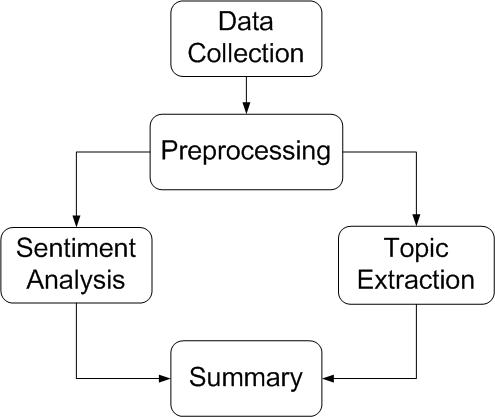
\includegraphics[width=.8\linewidth]{Process.jpg}
	\caption{Overview of approach}
	\label{fig:approachFig}
\end{figure}
Figure \ref{fig:approachFig} จะแสดงขั้นตอนทั้งหมดในการวิจัย โดยจะเริ่มตั้งแต่ 1. Data Collection 2. Prepossessing 3. Sentiment Analysis 4. Topic Extraction 5. Summary 
\subsection{Data Collection}

\begin{table}[h]
	\caption{no. of review in each app.}
	\label{table:NoOfReview}
	\centering
	\begin{tabular}{|c|r|}
		\hline
		Application & \multicolumn{1}{|c|}{no. of review} \\
		\hline
		Man Man & 1279\\
		\hline
		H-Tv & 691\\
		\hline
		K-mobile & 1055\\
		\hline
	\end{tabular}
\end{table}
เราได้รวบรวมข้อมูลความคิดเห็นของผู้ใช้งานจากโปรแกรมประเภทต่าง ๆ บน Google Play store โดยการรวบรวมจากบนหน้าเว็บไซต์สำหรับดาว์นโหลดโปรแกรมนั้น ๆ
โดยรวบรวมจากโปรแกรม "แม่น แม่น" (virtual keyboard), "H-Tv" (TV Online), "K-mobile" (Internet Mobile Banking) โดยเราได้รวบรวมข้อมูลในช่วง กุมภาพันธ์ 2015 - พฤษภาคม 2016 และ ช่วง มิถุนายน 2016 - สิงหาคม 2016 (นับจากวันที่ผู้ใช้งานแสดงความคิดเห็น) ซึ่งมีปริมาณข้อมูลตาม Table \ref{table:NoOfReview} โดยข้อมูลที่ผู้วิจัยได้รวบรวมมา ได้แก่ author, title, detail, rate, review-date ซึ่งแสดงตัวอย่างตาม Table \ref{table:review}

\begin{table*}[h]
	\caption{example of review}
	\label{table:review}
	\centering
	\begin{tabular}{|l|l|l|r|c|}
		\hline
		\multicolumn{1}{|c|}{author} &
		\multicolumn{1}{|c|}{title}&
		\multicolumn{1}{|c|}{review}&
		\multicolumn{1}{|c|}{rate}&
		\multicolumn{1}{|c|}{date}\\
		\hline
		โชคชัย มหาวงนันท์ & โชคชัย มหาวงศ์นันท์ & ใช้ได้ดีครับ & 5&10/04/2015\\
		\hline
		bie slow life &  & พักหลังนี่อัพบ่อยนะครับ & 4&09/19/2015\\
		\hline
		ornanohg Hongrrimon &  & ชอบค่ะใช้ง่าย มีตัวการ์ตูนให้ด้วย & 5&09/20/2015\\
		\hline
		Terdsak chompusri &  & เรียบง่ายแต่ใช้ได้ดีจริงๆครับชอบมาก & 5&09/22/2015\\
		\hline
		Worapote Panomauppatum & วรพจน์  พนมอุปถัมภ์ & ใช้ได้เยื่ยมมาก & 5&09/25/2015\\
		\hline
		Nate Makboon & เนตร มากบุญ & ดีมากครับ สะดวกดีแม่นสุดยอด & 5&09/24/2015\\
		\hline
	\end{tabular}
\end{table*}

%แต่สำหรับเจ้าของโปรแกรมนั้น ๆ สามารถนำข้อมูลเหล่านี้ออกมาได้จากหน้า console ของโปรแกรมนั้น ๆ ได้ทันที
\subsection{Prepossessing}
หลังจากที่เราได้ข้อมูลที่ต้องการแล้ว เราจะนำข้อมูลเหล่านั้นมาหา POS ก่อนเพื่อใช้ในการทำงานขั้นต่อไป แต่ก่อนที่เราจะหา POS ได้ เราจะต้องตัดประโยค และตัดคำก่อน
\subsubsection{sentence extraction}
เนื่องจากข้อมูลความคิดเห็น 1 ความคิดเห็นอาจจะไม่ได้มีเพียงประโยคเดียว ดังนั้นเราจึงจำเป็นต้องแบ่งประโยคออกมาเสียก่อน เนื่องจากประโยคภาษาไทยนั้นเราไม่มี pattern ที่ตายตัวในการแบ่งประโยคเหมือนอย่างภาษาอังกฤษ และในปัจจุบันมีคำสมัยใหม่เพิ่มขึ้นมาอีกมากมาย ทำให้ลำบากในการใช้เครื่องมือในการแบ่งประโยค อีกทั้งยังจำเป็นต้องใช้ corpus ที่มีข้อมูลของรูปประโยคที่ค่อนข้างมากเพื่อใช้ในการจำแนกประโยคต่าง ๆ ดังนั้นเราจึงใช้วิธี manual ในการแบ่งประโยค 

โดยเราใช้ pattern ในการแบ่งประโยคคือ\\ 
1. ถ้าเจอคำว่า "ครับ"/"ค่ะ" เราจะถือว่าเป็นการจบประโยค\\
2. ถ้าเจอคำว่า "แต่" เราจะถือว่าเป็นการขึ้นประโยคใหม่
\subsubsection{word segmentation}
เมื่อเราแบ่งประโยคเรียบร้อยแล้วเราจะนำประโยคที่ได้แต่ละประโยคมาตัดแยกคำเพื่อนำไปหา POS ต่อไป โดยในการตัดคำนั้นเราได้ใช้เครื่องมือที่ชื่อ LexTo ซึ่งพัฒนาโดย NECTEC เป็นซึ่งใช้วิธีการตัดคำแบบ longest matching 
ในการตัดคำ
\subsubsection{pos tagger}
เราหา pos ของคำโดยใช้ RDRPOStagger ซึ่งมี ORCHID เป็น corpus สำหรับการคำนวน
\subsection{Sentiment Analysis}
ส่วนนี้เป็นการนำประโยคที่มีการกำหนด pos ของคำแล้วมา คำนวนหาทัศนคติของประโยค โดยสำหรับการหา sentiment ของคำในภาษาไทยนั้นยังไม่มี corpus ที่เผยแพร่ ดังนั้นเราจึงเลือกใช้ SentiWordNet \cite{SentiWordNet} ซึ่งเป็น corpus สำหรับหา sentiment ของคำในภาษาอังกฤษ 

ดังนั้นขั้นตอนแรกของการหา sentiment ของงานวิจัยนี้จึงเป็นการแปลคำศัพท์จากไทย-อังกฤษ โดยเราเลือกใช้ LEXiTRON \cite{LEXiTRON} เป็นพจนานุกรมในการแปลคำศัพท์ โดยการหาคำที่มี POS ตรงกัน ทำให้เราได้ synonym ภาษาอังกฤษ

ขั้นต่อมาเราจะนำ synonym ที่ได้มาหา sentiment ใน SentiWordNet โดยค่าของ sentiment ที่ได้จะอยู่ในช่วง [-1,1] ดังตัวอย่างใน Table \ref{table:Top10sentiword}
แต่เนื่องจากค่าที่ได้จาก SentiWordNet เราพบว่า คำบางคำ ที่ให้ความรู้สึกในเชิงลบของรูปประโยค มีค่าที่ได้เป็นบวก ดังนั้นเราจึงจำเป็นต้องสร้างลิสต์คำที่คาดว่าให้ความรู้สึกเชิงลบ แล้วนำมาเทียบกับ sentiment ที่ได้ ถ้า sentiment ที่ได้เป็นบวก เราจะกลับค่า sentiment นั้นให้เป็นลบแทน และในกรณีที่มีคำว่า "ไม่" นำหน้าคำ ๆ นั้น เราก็จะกลับค่า sentiment ของคำนั้นแทน

จากนั้นเราจะหาค่า sentiment ของประโยคโดยการนำค่า sentiment ทั้งหมดของประโยคนั้น ๆ มาเฉลี่ยเป็นคะแนนของประโยค
\subsection{Topic Extraction}
ส่วนนี้เป็นส่วนที่อธิบายถึงวิธีการหาหัวข้อของประโยค โดยเราใช้วิธี LDA ในการค้นหาหัวข้อ ซึ่งจะทำหลังจากการหา pos ของคำ
โดยเรากำหนดให้ number of topic ที่ต้องการเป็น 20 เนื่องจากเราไม่ทราบหัวข้อที่แน่นอน จากนั้นเราจะเลือกหัวข้อที่เหมาะสมออกมาจากหัวข้อทั้งหมดที่ได้
%not finish
\subsection{Summary}
หลังจากที่เราได้กลุ่มคำของ topic ต่าง ๆ และ sentiment ของประโยคแล้ว เราจะรวมรวบประโยคที่มีคำตรงกับในกลุ่มคำของ topic เพื่อนำมาแสดงถึงคะแนน sentiment ของ topic นั้น ๆ และนำคะแนนที่ได้มาหาค่า absolute maximum เพื่อแสดงถึง sentiment รวมของหัวข้อนั้น ๆ ว่าคะแนนเป็นบวก หรือเป็นลบ Table\ref{table:topicManMan} แสดงถึงตัวอย่างคะแนนที่ได้จากการวิจัย

นอกจากนี้เรายังสามารถแจกแจงได้ว่าแต่ละหัวข้อมี ประโยคที่มีทัศนคติเป็นบวก หรือเป็นลบ อยู่อย่างละกี่ประโยคได้อีกด้วย


\begin{table}[h]
	\renewcommand{\arraystretch}{1.3}
	\caption{Top 10 sentiment of each word in Man Man app}
	\label{table:Top10sentiword}
	\centering
	\begin{tabular}{|c|c|c|c|}
		\hline
		\multicolumn{2}{|c|}{negative} &
		\multicolumn{2}{|c|}{positive}\\
		\hline
		{\selectlanguage{thai}ลบ} & -0.33621 & {\selectlanguage{thai}น่ารัก} & 0.21843\\
		\hline
		{\selectlanguage{thai}เสียดาย} & -0.17095 & {\selectlanguage{thai}รัก} & 0.20107\\
		\hline
		{\selectlanguage{thai}เกลียด} & -0.16666 & {\selectlanguage{thai}เพลิน} & 0.17563\\
		\hline
		{\selectlanguage{thai}ดุ} & -0.15297 & {\selectlanguage{thai}ดี} & 0.16622\\
		\hline
		{\selectlanguage{thai}สายตายาว} & -0.12500 & {\selectlanguage{thai}สวย} & 0.16310\\
		\hline
		{\selectlanguage{thai}ขยายตัว} & -0.09566 & {\selectlanguage{thai}สุดยอด} & 0.15476\\
		\hline
		{\selectlanguage{thai}ห่วย} & -0.09071 & {\selectlanguage{thai}มันส์} & 0.15085\\
		\hline
		{\selectlanguage{thai}ปวด} & -0.07943 & {\selectlanguage{thai}ไว} & 0.12500\\
		\hline
		{\selectlanguage{thai}เสียใจ} & -0.07943 & {\selectlanguage{thai}ชอบ} & 0.12246\\
		\hline
		{\selectlanguage{thai}ไม่ดี} & -0.06995 & {\selectlanguage{thai}สนุก} & 0.10604\\
		\hline
	\end{tabular}
\end{table}


The goal of our work is to extract opinions and sentiments about mobile applications from user reviews written in Thai. The work hopes to help Thai users assesss mobile application without needing to read all reviews and to also help Thai developers pinpoint where they can improve their software products. To achieve the goal, we employ 5 steps as follows: 1. Data Collection 2. Prepossessing 3. Sentiment Analysis 4. Topic Extraction 5. Summary as shown in Figure \ref{fig:approachFig}. 

\begin{figure}[h]
	\centering
	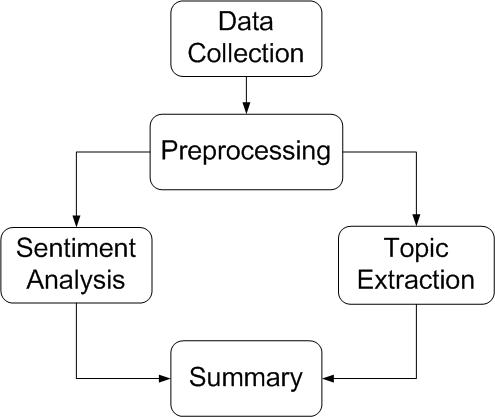
\includegraphics[width=.8\linewidth]{Process.jpg}
	\caption{Overview of approach}
	\label{fig:approachFig}
\end{figure}

We would like the entire process of analyzing raw user reviews to be automatic and accurate as much as possible, but it is not feasible to be 100\% automatic and accurate. To process raw user reviews, most of the process is done automatically but some parts need manual intervention. The following subsections describe these five steps and will also state whether the step is done automatically or manually. We also need to make some assumptions to make the process possible. For example, we assume that one sentence has one sentiment.

\subsection{Data Collection}

\begin{table}[h]
	\caption{Number of reviews in each application}
	\label{table:NoOfReview}
	\centering
	\begin{tabular}{|c|r|}
		\hline
		\textbf{Application} & \multicolumn{1}{|c|}{\textbf{No. of Reviews}} \\
		\hline
		Man Man & 1279\\
		\hline
		H-TV & 691\\
		\hline
		K-Mobile & 1055\\
		\hline
	\end{tabular}
\end{table}

\begin{table*}[h]
	\caption{Example of Reviews}
	\label{table:review}
	\centering
	\begin{tabular}{|l|l|l|c|c|}
		\hline
		\multicolumn{1}{|c|}{\textbf{Author}} &
		\multicolumn{1}{|c|}{\textbf{Title}} &
		\multicolumn{1}{|c|}{\textbf{Review}} &
		\multicolumn{1}{|c|}{\textbf{Rate}} &
		\multicolumn{1}{|c|}{\textbf{Date} (mm/dd/yyyy)}\\
		\hline
		{\selectlanguage{thai}โชคชัย มหาวงนันท์} & {\selectlanguage{thai}โชคชัย มหาวงศ์นันท์} & {\selectlanguage{thai}ใช้ได้ดีครับ} & 5&10/04/2015\\
		\hline
		bie slow life &  & {\selectlanguage{thai}พักหลังนี่อัพบ่อยนะครับ} & 4&09/19/2015\\
		\hline
		ornanohg Hongrrimon &  & {\selectlanguage{thai}ชอบค่ะใช้ง่าย มีตัวการ์ตูนให้ด้วย} & 5&09/20/2015\\
		\hline
		Terdsak chompusri &  & {\selectlanguage{thai}เรียบง่ายแต่ใช้ได้ดีจริงๆครับชอบมาก} & 5&09/22/2015\\
		\hline
		Worapote Panomauppatum & {\selectlanguage{thai}วรพจน์  พนมอุปถัมภ์} & {\selectlanguage{thai}ใช้ได้เยื่ยมมาก} & 5&09/25/2015\\
		\hline
		Nate Makboon & {\selectlanguage{thai}เนตร มากบุญ} & {\selectlanguage{thai}ดีมากครับ สะดวกดีแม่นสุดยอด} & 5&09/24/2015\\
		\hline
	\end{tabular}
\end{table*}


We have collected user reviews in Google Play Store from three mobile applications:
"{\selectlanguage{thai}แม่น แม่น}" or "Man Man" (a virtual keyboard), "H-TV" (online TV), "K-Mobile" (internet mobile banking). The user reviews collected are dated between February 2015 and August 2016. The number of user reviews collected for each application is shown in Table \ref{table:NoOfReview}. The information collected for each review includes author, title, detail, rate, and review date. Table \ref{table:review} shows examples of user reviews. 

The collection process is done automatically using a script written in JavaScript to retrieve user reviews automatically from the Google Play Store website. The user reviews are then stored in a database for further analysis.

\subsection{Prepossessing}

After user reviews have been collected, the next step is to perform sentence segmentation, word segmentation and part-of-speech tagging. 

\subsubsection{sentence extraction}
One user review can contain several sentences expressing opinions about various aspects or features. 
Since we make an assumption that one sentence has one sentiment, we need to distinguish different sentences in the review. Thai writing however makes it difficult because there is no formal sentence boundary like a period or a question mark in Engish writing. Spaces in Thai language can mark the end of a sentence or the end of a clause. Therefore, we cannot simply use spaces to indicate the end of sentences. Although there are several researches focusing on breaking Thai text into sentences, there are no tools that can easily be used. We therefore perform sentence segmentation manually. Once a tool is available, it can be applied to make this pre-processing step easier. 

\subsubsection{word segmentation}
As mentioned in Section \ref{Background}, we used LexTo\cite{LexTo} from NECTEC to perform word segmentation. LexTo can segment words very well if words are spelled correctly. However, processing raw user reviews is difficult because of the informal language and slangs used in the reviews. There are also many spelling errors, either accidentally or intentionally to emphasize the meaning such as "{\selectlanguage{thai}มากกกกกก}", causing the tool to segment words incorrectly. 

To ease the problem, LexTo allows us to add new vocabulary into the tool. However, with too many slangs including new ones and too many variations of misspelled words, it is not practical to add all of these into the tool. Today, more and more texts to be analyzed are written informally. It is more practical to find an automatic approach to deal with this problem rather than manually correctly these words so that the word segmentation tool can perform entirely correctly. In our work, we have added some common slangs and common misspelled into the tool to increase accuracy but are not able to cover all slangs and mispelled words. This step is therefore more automatic with the cost of less accuracy.

\subsubsection{POS tagger}

We use the RDRPOStagger tool\cite{RDRPOSTagger} with the ORCHID corpus\cite{ORCHID} for POS tagging. Since some slang and mispelled words are segmented incorrectly, the POS tagger tags those words as "unknown". In the sentiment analysis and topic modeling steps, only words tagged with nouns, verbs, and adjective/adverb are used. In addition, since one word can be tagged with more than one POS, this POS annotation is used to identify various meanings of one word. For example, the word "{\selectlanguage{thai}ฉัน}" has two meanings with different parts of speech. As a noun, it means "I". As a verb, it means "eat".

\subsection{Sentiment Analysis}
Once words in user reviews are tagged with parts of speech, sentiments in these reviews can be analyzed. Our work applies the lexicon-based approach. However, there is no resource that annotates each Thai word with sentiment scores. Therefore, the English SentiWordNet \cite{SentiWordNet} is used in combination with an electronic Thai-English dictionary called LEXiTRON \cite{LEXiTRON} developed by NECTEC.

To find score for each Thai word, our script automatically looks up in the LEXiTRON dictionary to retrieve its English word with the same part-of-speech tag. The next step is to look for sentiment score in SentiWordNet for the English word with the same POS. The sentiment score is between [-1,1] where negative number means negative sentiment and vice versa. Also, the higher the number means higher degree of negativity or positivity. Table \ref{table:Top10sentiword} shows examples of the sentiment scores. 

Besides assigning sentiment scores straightforwardly, further analysis is needed. For example, 
a word that is preceded with the word {\selectlanguage{thai}ไม่}, which means "no" or "not", will have its sentiment score flipped. In addition, some Thai words have more than one associated English words where these English words also have different sentiment scores. In this case, all sentiment scores are  averaged and then assigned to the Thai word. When sentiment scores are assigned to all nouns, verbs, adjectives, and adverbs in a sentence, the sentiment score for a sentence is calculated by averaging these sentiment scores.

Furthermore, we found that several negative sentences are assigned with positive score. Upon closer look, we found a pattern in these sentences where there is a word {\selectlanguage{thai}ชอบ} preceding with a negative verb such as "{\selectlanguage{thai}ชอบค้างบ่อยๆ}", which means the application often freezes. The word {\selectlanguage{thai}ชอบ} in Thai means "like", and if used in front of a verb, it also means "often". Since the POS tool tags {\selectlanguage{thai}ชอบ} as a verb which associates with the "like" meaning, its sentiment score is returned with a high positive number. This type of sentences is therefore incorrectly assigned with positive sentiment. Hence, we eliminate the word {\selectlanguage{thai}ชอบ} that precedes a verb to increase accuracy.


\begin{table}[h]
	\renewcommand{\arraystretch}{1.3}
	\caption{Top 10 sentiment of each word in Man Man app}
	\label{table:Top10sentiword}
	\centering
	\begin{tabular}{|c|c|c|c|}
		\hline
		\multicolumn{2}{|c|}{negative} &
		\multicolumn{2}{|c|}{positive}\\
		\hline
		word & sentiment & word & sentiment\\
		\hline
		{\selectlanguage{thai}ลบ} & -0.33621 & {\selectlanguage{thai}น่ารัก} & 0.21843\\
		\hline
		{\selectlanguage{thai}เสียดาย} & -0.17095 & {\selectlanguage{thai}รัก} & 0.20107\\
		\hline
		{\selectlanguage{thai}เกลียด} & -0.16666 & {\selectlanguage{thai}เพลิน} & 0.17563\\
		\hline
		{\selectlanguage{thai}ดุ} & -0.15297 & {\selectlanguage{thai}ดี} & 0.16622\\
		\hline
		{\selectlanguage{thai}สายตายาว} & -0.12500 & {\selectlanguage{thai}สวย} & 0.16310\\
		\hline
		{\selectlanguage{thai}ขยายตัว} & -0.09566 & {\selectlanguage{thai}สุดยอด} & 0.15476\\
		\hline
		{\selectlanguage{thai}ห่วย} & -0.09071 & {\selectlanguage{thai}มันส์} & 0.15085\\
		\hline
		{\selectlanguage{thai}ปวด} & -0.07943 & {\selectlanguage{thai}ไว} & 0.12500\\
		\hline
		{\selectlanguage{thai}เสียใจ} & -0.07943 & {\selectlanguage{thai}ชอบ} & 0.12246\\
		\hline
		{\selectlanguage{thai}ไม่ดี} & -0.06995 & {\selectlanguage{thai}สนุก} & 0.10604\\
		\hline
	\end{tabular}
\end{table}

\subsection{Topic or Feature Extraction}
In addition to sentiment analysis, we also want to pinpoint what topics or features users are talking about in the review. We use LDA, a topic modeling technique, to extract topics/features. We supplied only nouns, verbs, adjectives, and adverbs in all user reviews to the LDA Python tool. We specify the number of topics to be 20 because we do not know exactly how many features users are talking about in the reviews.

We then choose topics with high probabilities and also choose words within the topics with high probabilities.

%not finish

\subsection{Summary}
After sentences are annotated with sentiment scores and features are extracted, we summarize the information by assigning sentiment scores to the extracted features. The assigning process is done as follows. For each word belonging in a topic, we find all the sentences containing the word and collect all their sentiment scores. The absolute maximum sentiment score is then assigned to the topic.

%In addition, we also count how many sentencse with positive and negative scores for each topic so that developers can see in more details how much users like or dislike the features. 





\section{Result}\label{Result}

เราได้ตรวจสอบความถูกต้องของงานวิจัยโดยให้ผู้เชี่ยวชาญประเมินทัศนคติของประโยค ซึ่งจะได้ค่าความถูกต้องตาม Table \ref{table:f-measureSenti}
\begin{table}
	\caption{F-measure and Accuracy for sentiment analysis}
	\label{table:f-measureSenti}
	\centering
	\begin{tabular}{|l|r|r|r|r|}
		\hline
		\multicolumn{1}{|c|}{Application} &
		\multicolumn{1}{|c|}{Precision}&
		\multicolumn{1}{|c|}{Recall}&
		\multicolumn{1}{|c|}{F-measure} &
		\multicolumn{1}{|c|}{Accuracy} \\
		\hline
		Man Man & 0.5028 & 0.3189 & 0.3570 & 0.6110\\
		\hline
		H-Tv & 0.5208 & 0.2889 & 0.3366 & 0.4837 \\
		\hline
		K-mobile & 0.4535 & 0.2810 & 0.3240 & 0.5153 \\
		\hline
	\end{tabular}
\end{table}
\subsection*{Limitation}
เนื่องจากเรายังหาวิธีที่จะใช้ในการแบ่งประโยคที่ชัดเจนยังไม่ได้จึงทำให้การแบ่งประโยคนั้นอาจยังไม่ถูกต้อง รวมถึงคำบางคำ อาจจะเป็นคำสมัยใหม่ หรือภาษาวัยรุ่น ทำให้คำเหล่านี้ไม่มีอยู่ใน corpus ที่เราใช้งาน จึงเป็นเหตุให้เราอาจไม่สามารถหาทัศนคติของคำเหล่านี้ได้

และในการหา sentiment โดยการแปลภาษาไทย-อังกฤษ คำบางที่แปลได้ อาจแปลได้ไม่ตรงตามความต้องการของประโยคทั้งนี้เนื่องมาจาก การหา POS และ การพ้องรูปในภาษาไทย

อีกทั้งในเรื่องของการหาหัวข้อที่ไม่มีความแน่นอนของโปรแกรมต่าง ๆ จึงทำให้เรากำหนดจำนวนหัวข้อที่ต้องการไม่ได้



% An example of a double column floating figure using two subfigures.
% (The subfig.sty package must be loaded for this to work.)
% The subfigure \label commands are set within each subfloat command,
% and the \label for the overall figure must come after \caption.
% \hfil is used as a separator to get equal spacing.
% Watch out that the combined width of all the subfigures on a 
% line do not exceed the text width or a line break will occur.
%
%\begin{figure*}[!t]
%\centering
%\subfloat[Case I]{\includegraphics[width=2.5in]{box}%
%\label{fig_first_case}}
%\hfil
%\subfloat[Case II]{\includegraphics[width=2.5in]{box}%
%\label{fig_second_case}}
%\caption{Simulation results for the network.}
%\label{fig_sim}
%\end{figure*}
%
% Note that often IEEE papers with subfigures do not employ subfigure
% captions (using the optional argument to \subfloat[]), but instead will
% reference/describe all of them (a), (b), etc., within the main caption.
% Be aware that for subfig.sty to generate the (a), (b), etc., subfigure
% labels, the optional argument to \subfloat must be present. If a
% subcaption is not desired, just leave its contents blank,
% e.g., \subfloat[].


% An example of a floating table. Note that, for IEEE style tables, the
% \caption command should come BEFORE the table and, given that table
% captions serve much like titles, are usually capitalized except for words
% such as a, an, and, as, at, but, by, for, in, nor, of, on, or, the, to
% and up, which are usually not capitalized unless they are the first or
% last word of the caption. Table text will default to \footnotesize as
% the IEEE normally uses this smaller font for tables.
% The \label must come after \caption as always.
%
%\begin{table}[!t]
%% increase table row spacing, adjust to taste
%\renewcommand{\arraystretch}{1.3}
% if using array.sty, it might be a good idea to tweak the value of
% \extrarowheight as needed to properly center the text within the cells
%\caption{An Example of a Table}
%\label{table_example}
%\centering
%% Some packages, such as MDW tools, offer better commands for making tables
%% than the plain LaTeX2e tabular which is used here.
%\begin{tabular}{|c||c|}
%\hline
%One & Two\\
%\hline
%Three & Four\\
%\hline
%\end{tabular}
%\end{table}


%\begin{table*}[h]
%	\caption{example of result after pass POS tagger process}
%	\label{table:POSEx}
%	\centering
%	\begin{tabular}{|l|l|l|}
%		\hline
%		\multicolumn{1}{|c|}{sentense} &
%		\multicolumn{1}{|c|}{word segmentation} &
%		\multicolumn{1}{|c|}{POS}\\
%		\hline
%		ใช้ได้ดีครับ & 
%		ใช้ได้|ดี|ครับ| & 
%		ใช้ได้/npn ดี/vi ครับ/aff \\
%		\hline
%		เยี่ยม ดี เลิศ & 
%		เยี่ยม|ดี|เลิศ| & 
%		เยี่ยม/vt ดี/adv เลิศ/adv \\
%		\hline
%		พักหลังนี่อัพบ่อยนะครับ & 
%		พัก|หลัง|นี่|อัพบ่อย|นะ|ครับ| & 
%		พัก/vi หลัง/adj นี่/pdem อัพบ่อย/npn นะ/part ครับ/aff \\
%		\hline
%		ชอบค่ะใช้ง่าย มีตัวการ์ตูนให้ด้วย & 
%		ชอบ|ค่ะ|ใช้|ง่าย|มี|ตัว|การ์ตูน|ให้|ด้วย| & 
%		ชอบ/vt ค่ะ/aff ใช้/vt ง่าย/adv มี/vt ตัว/ncn การ์ตูน/ncn ให้/vpost ด้วย/adv \\
%		\hline
%		เรียบง่ายแต่ใช้ได้ดีจริงๆครับชอบมาก & 
%		เรียบง่าย|แต่|ใช้ได้|ดี|จริงๆ|ครับ|ชอบมาก| & 
%		เรียบง่าย/vi แต่/conj ใช้ได้/npn ดี/vi จริงๆ/adv ครับ/aff ชอบ/vt มาก/adv \\
%		\hline
%		ดีมากครับ สะดวกดีแม่นสุดยอด & 
%		ดีมาก|ครับ|สะดวก|ดี|แม่น|สุดยอด| & 
%		ดีมาก/npn ครับ/aff สะดวก/vi ดี/adv แม่น/vt สุดยอด/adj \\
%		\hline
%	\end{tabular}
%\end{table*}


%Table~\ref{table:topicManMan} displays aspects and sentiments after analyzing user reviews using our approach. Due to space limit, the table only shows results from \enquote{Man Man} application. In the table, the number of positive and negative sentences are also shown to give developers a sense of how often aspects were mentioned in user reviews. Figure~\ref{fig:graphmanman} visualizes the results from Table~\ref{table:topicManMan} with a graph and sorts aspects by sentiment scores. 

The sentiment scores shown in Table~\ref{table:topicManMan} has the highest positive and negative scores of 0.5153 and -0.5156, respectively. Upon examining SentiWordNet, we find that highest \textit{Pos} and \textit{Neg} scores are both 0.75 since the \textit{Obj} score is always non-zero. Since we use averages and absolute maximums when assigning scores to words and sentences, resulting sentiment scores for aspects should be in the range of [-0.75,0.75]. Thus, we can categorize the resulting scores to \textit{low}, \textit{medium}, \textit{high} when absolute scores are [0,0.25), [0.25, 0.5), [0.5,0.75], respectively. Hence, the sentiment score of 0.5153 and -0.5156 in Table~\ref{table:topicManMan} can be considered high positive and high negative. 

\begin{table}[h]
	\caption{20 topics/aspects discovered from Man Man user reviews}
	\label{table:topicManMan}
	\centering
	\begin{tabular}{|l|r|
			r|r|
		}
		\hline
		\multicolumn{1}{|c|}{\textbf{Topic/Aspect}} 
		& \multicolumn{1}{|c|}{\textbf{Sentiment}}
		& \multicolumn{1}{|c|}{\textbf{\# Pos. Sentences}}
		& \multicolumn{1}{|c|}{\textbf{\# Neg. Sentences}}
		\\
		\hline
		{\selectlanguage{thai}เปลี่ยน ภาษา} & 0.2770 
		& 35 & 9 
		\\
		\hline
		{\selectlanguage{thai}พัฒนา ยอด} & 0.2666 
		& 47 & 6 
		\\
		\hline
		sticker {\selectlanguage{thai}หน่อย ขยาย} & 0.2046 
		& 36 & 15 
		\\
		\hline
		{\selectlanguage{thai}สะดวก สวย} & 0.3926 
		& 84 & 13 
		\\
		\hline
		{\selectlanguage{thai}สายตา ขนาด ใหญ่} & 0.5153 
		& 143 & 26 
		\\
		\hline
		{\selectlanguage{thai}ยกเว้น ทำนาย} & 0.2315 
		& 19 & 2 
		\\
		\hline
		{\selectlanguage{thai}ปรับปรุง ยาก} & 0.2035
		 & 17 & 11 
		 \\
		\hline
		{\selectlanguage{thai}ปุ่ม หาย} & -0.5156 
		& 49 & 23 
		\\
		\hline
		{\selectlanguage{thai}ชอบ แม่น} & 0.3926 
		& 142 & 14 
		\\
		\hline
		{\selectlanguage{thai}สุดยอด ลอง} & 0.3926 
		& 145 & 12 
		\\
		\hline
		{\selectlanguage{thai}แป้น รวน} & -0.3352 
		& 24 & 9 
		\\
		\hline
		{\selectlanguage{thai}แก้ไข สี} & 0.2167 
		& 40 & 15 
		\\
		\hline
		{\selectlanguage{thai}พิมพ์ ง่าย} & 0.5153 
		& 201 & 12 
		\\
		\hline
		{\selectlanguage{thai}เสียง เสียดาย} & 0.4066
		 & 17 & 4 
		 \\
		\hline
		{\selectlanguage{thai}ปรับ ขนาด ค้าง} & 0.5153 
		& 63 & 13 
		\\
		\hline
		{\selectlanguage{thai}ปุ่ม แจ่ม ซับซ้อน} & -0.5156 
		& 30 & 17 
		\\
		\hline
		{\selectlanguage{thai}เพิ่ม อิโมจิ} & 0.4066 
		& 35 & 1 
		\\
		\hline
		{\selectlanguage{thai}เดา คำ} & -0.5156 
		& 44 & 9 
		\\
		\hline
		{\selectlanguage{thai}พิมพ์ พลาด} & 0.5153 
		& 68 & 11 
		\\
		\hline
		{\selectlanguage{thai}แป้น ใหญ่} & 0.3396 
		& 82 & 13 
		\\
		\hline
	\end{tabular}
\end{table}

\begin{figure}
	\centering
	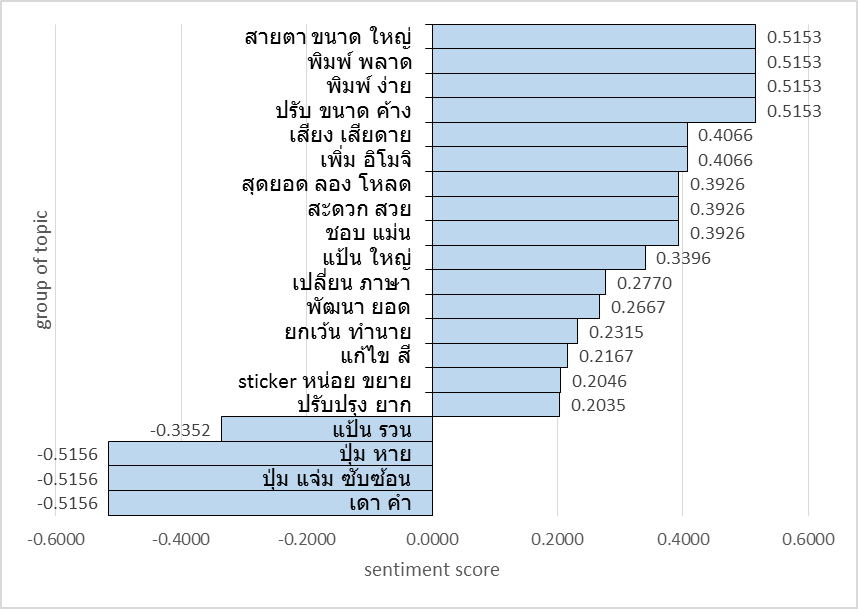
\includegraphics[width=0.9\linewidth]{graphmanman}
	\caption{Sentiment scores for topics/aspects from Man Man user reviews}
	\label{fig:graphmanman}
\end{figure}

%\begin{table}[h]
%	\caption{Evaluation results for sentence-level sentiments}
%	\label{table:f-measureSenti}
%	\centering
%	\begin{tabular}{|l|r|r|r|r|}
%		\hline
%		\multicolumn{1}{|c|}{\textbf{Application}} &
%		\multicolumn{1}{|c|}{\textbf{Precision}} &
%		\multicolumn{1}{|c|}{\textbf{Recall}} &
%		\multicolumn{1}{|c|}{\textbf{F-Measure}} &
%		\multicolumn{1}{|c|}{\textbf{Accuracy}} \\
%		\hline
%		Man Man & 0.5028 & 0.3189 & 0.3570 & 0.6110\\
%		\hline
%		H-TV & 0.5208 & 0.2889 & 0.3366 & 0.4837 \\
%		\hline
%		K-Mobile & 0.4535 & 0.2810 & 0.3240 & 0.5153 \\
%		\hline
%	\end{tabular}
%\end{table}

\begin{table}[!htbp]
	\caption{Evaluation results for sentiment analysis of extracted aspects}
	\label{table:f-measureTopic}
	\centering
	\begin{tabular}{|l|r|r|r|r|}
		\hline
		\multicolumn{1}{|c|}{\textbf{Application}} & 
		%\multicolumn{1}{|c|}{\multirow{2}{*}{application}} & 
		%\multicolumn{4}{|c|}{Topic} \\
		%\cline{2-5}
		%\multicolumn{1}{|c|}{} &
		\multicolumn{1}{|c|}{\textbf{Precision}} &
		\multicolumn{1}{|c|}{\textbf{Recall}} &
		\multicolumn{1}{|c|}{\textbf{F-Measure}} &
		\multicolumn{1}{|c|}{\textbf{Accuracy}} \\
		\hline
		Man Man & 0.7188 & 0.6538 & 0.6848 & 0.55\\
		\hline
		H-TV & 0.5252 & 0.5333 & 0.5293 & 0.5\\
		\hline
%		K-Mobile & 0.2368 & 0.45 & 0.3103 & 0.45\\
%		\hline
	\end{tabular}
\end{table}

%We evaluated our approach by asking one person not related our research to manually label sentiments whether a sentence is positive, negative, or neutral. This information is used as truth values to calculate precision, recall, and accuracy. Table~\ref{table:f-measureSenti} shows evaluation results of sentiment analysis on a sentence level.

We evaluated our approach by calculating precision, recall, F-measure, and accuracy using truth values from data labeled manually by one person not related to our research. To manually label data, the person was given aspects/topics generated from LDA in the topic modeling step and then labeled each aspect/topic with either positive or negative sentiment. Sentiment scores are not evaluated since it is highly subjective and can be difficult to analyze accuracy. Table~\ref{table:f-measureTopic} shows the evaluation results. The average F-measure from both applications is 0.6071. 

We have not evaluated whether the LDA produced accurate topics/aspects. For topic modeling, accuracy evaluation is very subjective and time-consuming. Different persons may have very different points of view on how to identify topics/aspects in large amount of data.  Since the LDA technique is widely known and used for topic modeling, we assume for now that results from LDA is acceptably accurate. Future work can be done to evaluate this step using similar human-intensive process as in Gunzmam and Laalej's work~\cite{userslikefeature}.

\subsection*{Limitation and Possible Future Works}
Our work still has some limitations such as limitations in word segmentations of informal texts, slangs, and misspelled words. This causes LEXiTRON and SentiWordNet not being able to find translations nor sentiment scores. Moreover, some words have several meanings, and LEXiTRON returns several translations. Thus, we do not get precise meanings nor precise sentiment scores. Possible future work is to create a Thai sentiment lexical resource to help Thai researchers perform sentiment analysis easier and more accurate.

For topic modeling, our work fixes a number of topics and therefore are not flexible or dynamic enough. For future work, we can allow the number to be configurable or determined dynamically from additional information extracted from applications such as a list of features or application size.

The evaluation process is still not ideal since only one person creates truth values. We will ask more persons to label data as our future work. More mobile applications can also be analyzed to expand our case studies. We can also make the approach into a tool where users specify a name of a mobile application and let the tool analyze and display results.


% An example of a double column floating figure using two subfigures.
% (The subfig.sty package must be loaded for this to work.)
% The subfigure \label commands are set within each subfloat command,
% and the \label for the overall figure must come after \caption.
% \hfil is used as a separator to get equal spacing.
% Watch out that the combined width of all the subfigures on a 
% line do not exceed the text width or a line break will occur.
%
%\begin{figure*}[!t]
%\centering
%\subfloat[Case I]{\includegraphics[width=2.5in]{box}%
%\label{fig_first_case}}
%\hfil
%\subfloat[Case II]{\includegraphics[width=2.5in]{box}%
%\label{fig_second_case}}
%\caption{Simulation results for the network.}
%\label{fig_sim}
%\end{figure*}
%
% Note that often IEEE papers with subfigures do not employ subfigure
% captions (using the optional argument to \subfloat[]), but instead will
% reference/describe all of them (a), (b), etc., within the main caption.
% Be aware that for subfig.sty to generate the (a), (b), etc., subfigure
% labels, the optional argument to \subfloat must be present. If a
% subcaption is not desired, just leave its contents blank,
% e.g., \subfloat[].


% An example of a floating table. Note that, for IEEE style tables, the
% \caption command should come BEFORE the table and, given that table
% captions serve much like titles, are usually capitalized except for words
% such as a, an, and, as, at, but, by, for, in, nor, of, on, or, the, to
% and up, which are usually not capitalized unless they are the first or
% last word of the caption. Table text will default to \footnotesize as
% the IEEE normally uses this smaller font for tables.
% The \label must come after \caption as always.
%
%\begin{table}[!t]
%% increase table row spacing, adjust to taste
%\renewcommand{\arraystretch}{1.3}
% if using array.sty, it might be a good idea to tweak the value of
% \extrarowheight as needed to properly center the text within the cells
%\caption{An Example of a Table}
%\label{table_example}
%\centering
%% Some packages, such as MDW tools, offer better commands for making tables
%% than the plain LaTeX2e tabular which is used here.
%\begin{tabular}{|c||c|}
%\hline
%One & Two\\
%\hline
%Three & Four\\
%\hline
%\end{tabular}
%\end{table}


%\begin{table*}[h]
%	\caption{example of result after pass POS tagger process}
%	\label{table:POSEx}
%	\centering
%	\begin{tabular}{|l|l|l|}
%		\hline
%		\multicolumn{1}{|c|}{sentense} &
%		\multicolumn{1}{|c|}{word segmentation} &
%		\multicolumn{1}{|c|}{POS}\\
%		\hline
%		ใช้ได้ดีครับ & 
%		ใช้ได้|ดี|ครับ| & 
%		ใช้ได้/npn ดี/vi ครับ/aff \\
%		\hline
%		เยี่ยม ดี เลิศ & 
%		เยี่ยม|ดี|เลิศ| & 
%		เยี่ยม/vt ดี/adv เลิศ/adv \\
%		\hline
%		พักหลังนี่อัพบ่อยนะครับ & 
%		พัก|หลัง|นี่|อัพบ่อย|นะ|ครับ| & 
%		พัก/vi หลัง/adj นี่/pdem อัพบ่อย/npn นะ/part ครับ/aff \\
%		\hline
%		ชอบค่ะใช้ง่าย มีตัวการ์ตูนให้ด้วย & 
%		ชอบ|ค่ะ|ใช้|ง่าย|มี|ตัว|การ์ตูน|ให้|ด้วย| & 
%		ชอบ/vt ค่ะ/aff ใช้/vt ง่าย/adv มี/vt ตัว/ncn การ์ตูน/ncn ให้/vpost ด้วย/adv \\
%		\hline
%		เรียบง่ายแต่ใช้ได้ดีจริงๆครับชอบมาก & 
%		เรียบง่าย|แต่|ใช้ได้|ดี|จริงๆ|ครับ|ชอบมาก| & 
%		เรียบง่าย/vi แต่/conj ใช้ได้/npn ดี/vi จริงๆ/adv ครับ/aff ชอบ/vt มาก/adv \\
%		\hline
%		ดีมากครับ สะดวกดีแม่นสุดยอด & 
%		ดีมาก|ครับ|สะดวก|ดี|แม่น|สุดยอด| & 
%		ดีมาก/npn ครับ/aff สะดวก/vi ดี/adv แม่น/vt สุดยอด/adj \\
%		\hline
%	\end{tabular}
%\end{table*}




\section{Conclusion}\label{Conclusion}

งานวิจัยนี้ ได้เสนอแนวคิดในการหาหัวข้อและทัศนคติของโปรแกรมในโทรศัพท์เคลื่อนที่ ด้วยวิธีการ NLP และ Topic modeling ซึ่งผลลัพธ์ที่ได้อาจจะยังไม่น่าพอใจมากนัก แต่ยังสามารถนำมาเป็นแนวทางในการวิจัยต่อ ๆ ไปได้


%This paper presented an approach to analyze user reviews of mobile applications to discover aspects or features and their associated sentiments users talked about. The approach applied natural language processing steps such as word segmentation, part-of-speech tagging as well as a topic modeling and sentiment analysis techniques. The result is still not perfectly accurate nor fully automatic because of several limitations discussed in the paper. Several possible futures also discussed to make the approach more automatic and accurate.



% conference papers do not normally have an appendix


% use section* for acknowledgment
%\section*{Acknowledgment}
%
%The authors would like to thank...



% trigger a \newpage just before the given reference
% number - used to balance the columns on the last page
% adjust value as needed - may need to be readjusted if
% the document is modified later
%\IEEEtriggeratref{8}
% The "triggered" command can be changed if desired:
%\IEEEtriggercmd{\enlargethispage{-5in}}

% references section
% can use a bibliography generated by BibTeX as a .bbl file
% BibTeX documentation can be easily obtained at:
% http://mirror.ctan.org/biblio/bibtex/contrib/doc/
% The IEEEtran BibTeX style support page is at:
% http://www.michaelshell.org/tex/ieeetran/bibtex/
\bibliographystyle{IEEEtran}
% argument is your BibTeX string definitions and bibliography database(s)
\bibliography{paperref}
%
% <OR> manually copy in the resultant .bbl file
% set second argument of \begin to the number of references
% (used to reserve space for the reference number labels box)


%\begin{thebibliography}{1}
%	
%%	\bibitem{IEEEhowto:kopka}
%%	H.~Kopka and P.~W. Daly, \emph{A Guide to \LaTeX}, 3rd~ed.\hskip 1em plus
%%	0.5em minus 0.4em\relax Harlow, England: Addison-Wesley, 1999.
%	\bibitem{SentiWordNet}
%	S.~Baccianella and et al., "SentiWordNet 3.0: An Enhanced Lexical Resource for Sentiment Analysis and Opinion Mining," \emph{LREC.}, vol. 10, 2010, pp. 2200-2204.
%	
%	\bibitem{145Q} A.~Begel and T.~Zimmermann, "Analyze This! 145 Questions for Data Scientists in Software Engineering," in \emph{Proceeding of the 36th International Conference on Software Engineering}, ACM, 2014, pp. 12-23.
%	
%	\bibitem{LDA} D.~M. Blei and M.~I. Jordan, "Latent dirichlet allocation," \emph{Journal of machine Learning reserch}, vol. 3, 2003, pp.993-1022.
%	
%	\bibitem{featurethaiwordseg}
%	P.~Charoenpornsawat, "Feature-Based Thai Word Segmentation," M.S. thesis, Dept. Comp. Eng., Chulalongkorn Univ., Bangkok, Thailand, 1999.
%	
%	\bibitem{ar-miner}
%	N.~Chen and et al., "Ar-Miner: Mining Informative Reviews for Developers from Mobile App Marketplace," in \emph{Proceedings of the 36th International Conference on Software Engineering}, ACM, 2014, Hyderabad, India, pp. 767-778.
%	
%	\bibitem{basicemotion}
%	P.~Ekman, "An Argument for Basic Emotions," \emph{An Argument for Basic Emotions}, vol. 6, no. 3-4, 1992, pp. 169-200.
%	
%	\bibitem{userslikefeature}
%	E.~Guzman and W.~Maalej, "How Do Users Like This Feature? A Fine Grained Sentiment Analysis of App Reviews," in \emph{Proceedings of the 22nd International Conference on Requirements Engineering (RE)}, IEEE, 2014,pp. 153-162.
%	
%	\bibitem{thaiopinionmininghotel}
%	C.~Haruechaiyasak and A.~Kongthon, "Contructing Thai Opinion Mining Resource : A Case Study on Hotel Reviews," in \emph{Proceedings of the 8th Workshop on Asian Language Resources}, 2010, pp. 64-71. 
%	
%	\bibitem{ssense}
%	C.~Haruechaiyasak and A.~Kongthon, "S-Sense : A Sentiment Analysis Framework for Social Media Sensing," in \emph{6th International Joint Conference on Natural Language Processing}, 2013, pp. 6-13.
%	
%	\bibitem{emotioninthai}
%	P.~Inrak and S.~Sinthupinyo, "Applying Latent Senmantic Analysis to Classify Emotions in Thai Text," in \emph{Proceedings of the 2nd International Conference on Computer Engineering and Technology (ICCET)}, IEEE, vol. 6, 2010, pp. 450-454.
%	
%	% รอจัด format
%	\bibitem{paragraphextract}
%	C.~Jaruskulchai and C.~Kruengkrai, "A Practical Text Summarizer by Paragraph Extraction for Thai," in \emph{Proceedings of the 6th international workshop on Information retrieval with Asian language}, 2003, pp. 9-16.
%	
%	\bibitem{asum}
%	Y.~Jo and A.~H. Oh., "Aspect and Sentiment Unification Model for Online Review Analysis,", in \emph{Proceedings of the 4th ACM international conference on Web search and data mining}, ACM, Hong Kong, China, 2011, pp. 815-824.
%	
%	\bibitem{thaiwordfilter}
%	A.~Kawtrakul, and et al., "A Statistical Approach to Thai Word Filtering," in \emph{The 2nd symposium on natural language processing}, Bangkok, 1997.
%	
%	\bibitem{surveyopinionmining}
%	B.~Liu, "A Survey of Opinion Mining and Sentiment Analysis," \emph{Mining Text Data}, Springer, 2012, pp. 415-463. 
%	
%	\bibitem{cosine similarity}
%	C.~D. Manning, and et al. (2015, July 27) An Introduction to Information Retrieval, [Online]. Available: http://nlp.stanford.edu/IR-book/pdf/irbookonlinereading.pdf
%	
%	\bibitem{LexTo}
%	National Electronics and Computer Technology Center. (2015, July 27) Lexto: Text Lexeme Tokenizer, [Online]. Available: http://www.sansarn.com/lexto
%	
%	\bibitem{LEXiTRON}
%	National Electronics and Computer Technology Center. (2015, July 27) Lexitron, [Online]. Available: http://lexitron.nectec.or.th/2009\_1 
%	
%	\bibitem{RDRPOSTagger}
%	D.~Q. Nguyen and et al. "RDRPOSTagger: A Ripple Down Rules-based Part-Of-Speech Tagger," in \emph{Proceedings of the Demonstrations at the 14th Conference of European Chapter of the Association for Computational Linguistics}, 2014, Gothenburg, Sweden, pp. 17-20.
%	
%	\bibitem{EMNB}
%	K.~Nigam and et al., "Text Classification from Labeled and Unlabeled Documents Using EM," \emph{Machine Learning}, vol. 39, no. 2-3, 2000, pp. 103-134.
%	
%	\bibitem{NLTK}
%	NLTK Project. (2015, July 27) Natural Language Toolkit, [Online]. Available: http://www.nltk.org
%	
%	\bibitem{syllableseparator}
%	Y.~Poovarawan and W.~Imarrom, "Thai Syllable Separator by Dictionary," in \emph{Proceedings of the 9th Annual Meeting on Electrical Engineering of the Thai Universities}, Khonkaen, Thailand, 1986, pp. 14.
%	
%	\bibitem{wordsegforthai}
%	V.~Sornlertlamvanich, "Word Segmentation for Thai in Machine Translation System," in \emph{Machine Translation}, NECTEC, Bangkok, Thailand, 1993, pp. 50-56.
%	
%	\bibitem{ORCHID}
%	V.~Sornlertlamvanich and et al. "ORCHID: Thai Part-of-Speech Tagged Corpus," \emph{National Eletronics and Computer Technology Center Technical Report}, pp. 5-19, 1997.
%	
%	\bibitem{SentiStrength}
%	M.~Thelwall and et al., "Sentiment in Short Strength Detection Informal Text," \emph{Journal of the American Society for Information Science and Technology}, vol. 61, no. 12, 2010, pp. 2544-2558. 
%	
%	\bibitem{NAiST}
%	P.~Varasai and et al., "Building an Annotated Corpus for Text Summarization and Question Answering," in \emph{Proceedings of the International Conference on Language Resoureces and Evaluation}, Marakech, Morocco, 2008, pp. 3427-3434.
%	
%	\bibitem{keywordmining}
%	P.~M. Vu and et al., "Mining User Opinions in Mobile App Reviews: A Keyword-Based Approach," in \emph{Automated Software Engineering (ASE)}, IEEE, 2015, pp. 749-759.
%	
%\end{thebibliography}



% that's all folks
\end{document}


